\documentclass{article}
\usepackage{graphicx}
\usepackage{amsmath}
\usepackage{csvsimple}
\usepackage{adjustbox}
\usepackage{listings}
\usepackage{color}
\usepackage{geometry}
\geometry{
    letterpaper,
    left=1in,
    right=1in,
    top=1in,
    bottom=1in
}

\definecolor{codegreen}{rgb}{0,0.6,0}
\definecolor{codegray}{rgb}{0.5,0.5,0.5}
\definecolor{codepurple}{rgb}{0.58,0,0.82}
\definecolor{backcolour}{rgb}{1,1,1}
\definecolor{gray}{rgb}{0.75, 0.75, 0.75}

\lstdefinestyle{codestyle}{
    backgroundcolor=\color{backcolour},
    commentstyle=\color{codegreen},
    keywordstyle=\color{magenta},
    numberstyle=\tiny\color{codegray},
    stringstyle=\color{codepurple},
    basicstyle=\footnotesize,
    breakatwhitespace=false,
    breaklines=true,
    keepspaces=true,
    numbers=left,
    numbersep=5pt,
    showspaces=false,
    showstringspaces=false,
    showtabs=false,
    tabsize=4
}

\begin{document}

\title{Linear-Time Backbone Determination in a Wireless Sensor Network}
\author{Jake Carlson}
\date{April 23, 2018}
\maketitle

\abstract
A report on implementing algorithms to partition a random geometric graph into bipartite subgraphs. Three different graph geometries are explored: unit square, unit disk, and unit sphere. Nodes are uniformly distributed across the geometry. Then the edges are determined and the vertices are colored using smallest-last vertex ordering and greedy graph coloring. Once coloring has been used to determine the independent color sets, the combinations of the largest are processed to find the largest backbones. All algorithms used in this report are implemented to run in linear time.
\newpage

\tableofcontents
\lstlistoflistings
\newpage

\section{Executive Summary}

    \subsection{Introduction}
    Random geometric graphs (RGGs) are useful for simulating wireless sensor networks placed in different topologies. This project examines three different geometries: Square, Disk, and Sphere. The user supplies parameters for how many nodes they want in the network and how many connections they want for each node. Then, the simulation finds the average radius needed for that number of connections, determines the edges in the graph, colors the graph to find independent sets, pairs the four largest independent sets to find the largest bipartite subgraphs, and cleans these bipartites to find the major component, or backbone, of each bipartite. The cleaning ensures that there are no singular points of failure that could cause the network to become disconnected. In other words, each backbone exists so that there are multiple paths between any two nodes in the backbone.
    \par
    This creates network backbones from the random geometric graphs that are highly reliable and allow the largest number of wireless sensors to connect to it in only one hop. Additionally, the linear time implementation of this simulation ensures efficient running time regardless of the input size. The organization of the code base also makes it easy to implement new topologies by subclassing the main Topology class that implements all of the algorithms needed to determine the backbone.
    \par
    All of the code used for this project, including the graphical display of the generated graphs at each stage in the backbone determination process, can be found here:

    \begin{center}
        \texttt{https://github.com/jakecarlson1/sensor-network}
    \end{center}

    \subsection{Environment Description}
    The data structures and topologies for this simulation are implemented in Python2.7. The graphics are generated using Processing.py \cite{processing}. All development and benchmarking has been done on a 2014 MackBook Pro with a 3 GHz Intel Core i7 processor and 16 GB of DDR3 RAM running macOS High Sierra 10.13.4. I used a MacBook Pro and the macOS operating system becuase it is Unix based and is easy to develop in.
    \par
    Processing offers an easy to use API for drawing and rendering shapes two- and three-dimensions. The Processing.py implementation allows the use of the Python programming languages and libraries.
    \par
    A separate data generation script was used to generate the summary tables (Tables \ref{tab1}, \ref{tab2}, \ref{tab3}). Because these benchmarks were run in a separate script, the timing does not measure the time required to draw the graphs using Processing. The figures were generated using the matplotlib library \cite{matplotlib}. This library, and a variety of others, could not be imported into Processing.py because the jython interpreter used by Processing only accepts libraries written in raw Python.
    \par
    The different geometries were implemented in a stand alone Python file and imported into the Processing.py script or the data generation script, depending on what was being run. These classes can then be used directly by Processing or the data generation script. Because there is no intermediary file to hold the generated nodes and edges, there is no additional disk space needed to run the simulation. Everything can be done in system memory managed by Processing.

    \begin{center}
        \begin{table}[h]
            \centering
            \begin{adjustbox}{width=1\textwidth}
                \csvautotabular{./data/benchmark-data-1.csv}
            \end{adjustbox}
            \caption{Benchmarks for generating RGGs. A: input average degree, r: node connection radius}
            \label{tab1}
        \end{table}
    \end{center}

    \begin{center}
        \begin{table}[h]
            \centering
            \csvautotabular{./data/benchmark-data-2.csv}
            \caption{Benchmarks for coloring RGGs}
            \label{tab2}
        \end{table}
    \end{center}

    \begin{center}
        \begin{table}[h]
            \centering
            \begin{adjustbox}{width=1\textwidth}
                \csvautotabular{./data/benchmark-data-3.csv}
            \end{adjustbox}
            \caption{Benchmarks for backbone determination}
            \label{tab3}
        \end{table}
    \end{center}

\section{Reduction to Practice}

    \subsection{Data Structure Design}
    The primary data structure used for this project is an adjacency list. However, to allow for constant time lookup of edges of a node, a Python dictionary is used where the keys are nodes and the values are a list of indices of adjacent nodes in the original list of nodes. The space needed by the adjacency list is $\Theta(|V| + 2|E|)$. Two entries are used for each edge because they are undirected. This is superior to the adjacency matrix data structure which would require $\Theta(|E|^2)$ space.
    \par
    In order to make this project maintainable as it is developed along the semester, the object-oriented capabilities of Python are used to design the different geometries. First, a Topology class is defined that creates the interface Processing uses to draw the graphs. This base class implements all of the methods needed for node placement and edge detection in 2D graphs. Then, three subclasses are created: Square, Disk, and Sphere.
    \par
    The Square and Disk topologies simply need to override the methods for generating nodes and calculating the node radius needed for the desired average degree. The Sphere subclass needs to override a few additional functions because it exists in a 3D space. Other than the methods for generating nodes and calculating the node radius, it also needs to override the function used to draw the graph so that Processing will render the graph properly in 3D.

    \subsection{Algorithm Descriptions}

        \subsubsection{Node Placement}
        A different node placement algorithm is required for each of the geometries. For the Square, the coordinates for each node are generated as two random numbers taken from a uniform distribution on the range $[0,1]$. All of these points are guaranteed to be in the unit square.
        \par
        For the Disk, a similar method is used. The coordinates for nodes are randomly sampled from a uniform distribution; however, if a node has a distance from the center of the Disk greater than the radius of 1, the coordinates for that node are resampled.
        \par
        For the Sphere a different method must be used so that all of the nodes are placed on the surface of the Sphere and the volume is vacant. For this geometry, the following equations are used:

        \begin{align}
            x &= \sqrt{1-u^2}\cos\theta \\
            y &= \sqrt{1-u^2}\sin\theta \\
            z &= u
        \end{align}

        where $\theta \in [0,2\pi]$ and $u \in [-1,1]$. This is guaranteed to uniformly distribute nodes on the surface area of the sphere \cite{spherepoints}.
        \par
        All of these algorithms can be solved in $\Theta\left(|V|\right)$ where because each node only needs to be assigned a position once.

        \subsubsection{Edge Determination}
        To calculate the node connection radius needed to achieve the desired average connection, the ratio of node coverage to the total area can be used. This ratio must equal the ratio of the total number of nodes to the average degree, or:

        \begin{align}
            \frac{A_{geometry}}{A_{node}}= \frac{Num\,Nodes}{Avg\,Deg}
        \end{align}

        Applying this to each geometry only requires filling in the equation for the area of the geometry and the connection area. This is straight forward for the square and disk. The geometry areas are given by $R^2 = 1$ and $\pi R^2 = \pi$ respectively since these are the unit square and circle. The sphere is slightly more complicated. Since nodes should only be able to connect over the surface of the sphere (following arcs), the connection area is to be taken as the surface area of the spherical cap such that the arc of the cap is twice the length of the connection distance. In other words, a node placed on the surface of the sphere in the center of a spherical cap can connect to any other node that falls in that spherical cap. The equation for the area of the spherical cap is given by

        \begin{align}
            S_{cap} = \pi (a^2 + h^2)
        \end{align}

        where $a$ is the distance from the midpoint of the base of the cap to the edge of the base, and $h$ is the distance from the midpoint of the base to the top of the cap (where the node would be) \cite{spherecap}. If we connect these points with a third variable, $x$, such that $x$ is the actual distance from the node to the edge of its connection area, the Pythagorean theorem can be used to substitute in $x^2$ for $a^2 + h^2$. The equation for the node connection radius of the unit sphere then looks identical to that of the unit circle. The final list of equations used to calculate node connection radius for a desired average degree are given in Table \ref{tab4}.

        \begin{center}
            \begin{table}[h]
                \centering
                \begin{tabular}{|c|c|c|c|}
                    \hline
                    Geometry & Geometry Area & Node Area & r \\
                    \hline
                    Square & 1 & $\pi r^2$ & $r = \sqrt{\frac{Average\,Deg}{\pi \times Num\,Nodes}}$ \\
                    Disk & $\pi$ & $\pi r^2$ & $r = \sqrt{\frac{Average\,Deg}{Num\,Nodes}}$ \\
                    Sphere & $4\pi$ & $\pi r^2$ & $r = 2 \times \sqrt{\frac{Average\,Deg}{Num\,Nodes}}$ \\
                    \hline
                \end{tabular}

                \caption{Equations for node conneciton radius}
                \label{tab4}
            \end{table}
        \end{center}

        There are several methods for finding the edges in the graph, but this project uses the cell method which is capable of finding all of the edges in the graph in linear time \cite{rggpartition}. This method places the nodes into cells of area $r \times r$ based on their position in the topology. When the edge detection runs, each node needs to be visited once, but only the cell the node populates and the neighboring cells need to be searched for connections.

        \subsubsection{Graph Coloring}
        Two algorithms are used for coloring the graphs. The first is smallest-last vertex ordering, which sorts the vertices based on the number of degrees they have. The second is the greedy graph coloring algorithm.
        \par
        Smallest-last vertex ordering is used to order the nodes for coloring. The steps to this algorithm are as follows \cite{slv}:

        \begin{enumerate}
            \item Initialize a representation of your target graph
            \item Find the vertex $v_j$ of minimum degree in your representation
            \item Update your representation to simulate deleting $v_j$
            \item If there are still vertices in the representation, return to step 1, otherwise terminate with the sequence of vertices removed
        \end{enumerate}

        This algorithm is linear if each of the above steps is linear. Step 1 is linear if we can build a representation of the graph in linear time. For this, we can use an array of buckets, where each bucket holds the vertices that have the same number of edges as the position of the bucket in the array of buckets. To build this data structure, each node only needs to be visited once, making this linear in both space and time. Next, finding the vertex of minimum degree simply requires finding the lowest index bucket that has a node. This is bounded by the number of buckets, which is bounded by the number of nodes, making Step 2 linear. Next, we have to update the representation of the graph. To do this, we have to look at each node that shares an edge with $v_j$ and move it to the bucket for nodes with one fewer degree. This requires traversing the list of edges for $v_j$ which means Step 3 is linear. Since this is repeated for each node, the runtime of this program is $\Theta\left(|E| + |V|\right)$ and the space needed is $\Theta(|V|)$.
        \par
        After this, a single traversal of the smallest-last vertex ordering is needed to color the graph. As we traverse this list, we check to see if the nodes before it (that are already colored) share an edge with the current node. The node can then be colored with any color it does not share an edge with or, if it shares an edge with all currently used colors, it is assigned a new color. This algorithm is also linear. Each node needs to be visited once and when a node is visited, all previous nodes are checked to see if they are in the edge list of the current node. Because we used smallest last vertex ordering, as we have to check more and more nodes, we get to check fewer and fewer edges. This makes the greedy coloring algorithm $O(|V| + |E|)$.

        \subsubsection{Backbone Determination}
        Several algorithms are needed for determining the most suitable backbones for the wireless sensor network. First, the four largest independent sets are paired with each other to generate the largest bipartite subgraphs for the random geometric graph. These bipartites are bound to have minor components that are not connected to the major component, and blocks that are only connected by bridges. These nodes need to be removed in order for the backbone to be considered reliable. Once all of these nodes have been removed from the bipartite, the backbone has been determined. Then, the two backbones with the largest size are selected and their domination (ratio of nodes connected to the backbone) and number of faces (for the sphere topology) are calculated.
        \par
        The largest independent sets are the largest color sets given by smallest-last vertex coloring. These will be the first four color sets when greedy coloring is used on a sequence of nodes sorted in smallest-last order. The combination of these four independent sets must be taken to find the six largest bipartite subgraphs.
        \par
        The bipartite subgraphs need to be cleaned up in order to measure the size and coverage area of the backbone. This can be done by first removing all of the tails in the graph, which are sequences of nodes coming off of a component where the end node has degree one, and all nodes in between have degree two. Then, the major component needs to be determined, which is the component with the largest order. Once the largest component is determined, the minor blocks and the bridges connecting them to the major component need to be removed. A bridge is similar to a tail; it is a chain of edges that, if removed from the graph would increase the number of connected components. These features need to be removed because they do not provide reliability to the wireless sensor network. If a single one of these node were to fail, a portion of the graph would become disconnected from the remaining backbone. This creates a single point of failure that should not occur in a network backbone.
        \par
        Each of these algorithms can be implemented in linear time. Taking the combinations of the four largest independent color sets can be done by building a bipartite subgraph for each combination where the nodes are copied from the two color sets that make up the bipartite. Each bipartite will then be built in $\Theta(2|V|)$ time and $\Theta(2|V|)$ space where $|V|$ is the number of nodes in each color set. Since there are six ways to choose two items from a set of 4, this runs six times, resulting in $\Theta(12|V|)$ space and time usage for building all of the bipartites.
        \par
        The tails then need to be removed. This can be done by repeatedly removing all nodes with a degree of one. This will repeatedly remove the last node in the tail until the only remaining node is the node that connected the tail to its component. This will also remove any minor components that consist of a thin chain of nodes with no cycles. This is similar to smallest-last vertex ordering, except the deletion of nodes from the graph stops when there are no more nodes in the bucket for degree one. Since this algorithm is based off of smallest-last vertex ordering, and slvo ran in $\Theta\left(|E| + |V|\right)$, this is bounded above by smallest-last vertex ordering, $O\left(|E| + |V|\right)$. However, since the bipartite could have no tails in it, the lower bound of the runtime is $\Omega(|V|)$ which is the amount of time needed to place nodes in their respective buckets based on how many edges they have in the bipartite. Regardless, this will require $\Theta(|V|)$ space to create a representation of the bipartite that can be deleted from.
        \par
        Next, the major component needs to be determined. This can be done with breadth-first search. BFS will traverse the entire graph, counting the number of nodes that can be reached from some start node. If an entire component has been explored from some start node, and there are still unvisited nodes in the graph, BFS will pick a new start node and begin searching from there. By counting the number of nodes connected to each start node, the size of each component can be determined. The major component can be determined by taking the max of these sizes. BFS works with a queue of nodes to search. At the start of an iteration, the current node is removed from the front of the queue, and all of its neighbors are added to the queue, if they have not already been visited. Since each node is only visited once, the runtime for BFS is $\Theta(|V| + |E|)$. BFS operates in-place on the graph, but a parallel array to the array of nodes is needed to remember if a node has been visited or not. This requires $\Theta(|V|)$ space and time to initialize. All together, this algorithm runs $Theta(2|V| + |E|)$ time.
        \par
        Next, the bridges need to be removed from the major components. This can be done by modifying depth-first search to check for back-edges to nodes. If some node and its edges are being searched, it is a bridge if and only if none of the decedents of the nodes connected to the current node have a back-edge to the current node or any of its ancestors. Back-edges can be checked by maintaining a list of visit times given by the DFS algorithm (tin), and a list of the minimum entry time of any ancestor (fup). If the current node's neighbors have decedents with an earlier entry time, then they must have a back-edge to that node. If they have a back-edge with the current node, the minimum entry time of the ancestors would be the current time. If the minimum entry time of the neighbor's ancestors is greater than the current time, it must be a bridge. This is codified in the following formula \cite{bridges}:

        \begin{align}
            fup[v] = min
            \begin{cases}
                tin[v] \\
                tin[p]\,\text{for all $p$ for which $(v,\,p)$ is a back edge} \\
                fup[to]\,\text{for all $to$ for which $(v,\,to)$ is a tree edge}
            \end{cases}
        \end{align}

        Given this formula, the current edge $(v,\,to)$ is a bridge if and only if $fup[to] > tin[v]$ in the DFS tree. DFS runs in $\Theta(|V| + |E|)$ and the book-keeping data structures add a total space requirement of $\Theta(2|V|)$.
        \par
        Once the bridges have been found, the graph needs to be simulated to have them removed, and the resulting connected components need to be searched again for the major component. BFS can be used again, where if an edge is encountered that is in the set of bridge edges, the neighbors to the current node are not pushed into the queue. Using BFS again has a time and space requirements $Theta(2|V| + |E|)$ time and $\Theta(|V|)$ space.
        \par
        With the bridges removed, the major component in each graph has been determined and all single points of failure that could result in the disconnection of backbone nodes have been removed. It is then time to determine the two largest backbones for further evaluation. The size of the backbones (the number of edges) can be determined in linear time by traversing all of the nodes in the backbone and counting the edges that are shared with other nodes in the backbone. This runs in-place on the backbone representation in $\Theta(|V| + |E|)$ time for each backbone that needs to have its size calculated.
        \par
        The domination of the two largest backbones needs to be calculated. Finding the number of nodes connected directly to the backbone is equivalent to finding the number of nodes that are not connected to the backbone. This can be done by traversing all nodes that are not part of the backbone and, for each of their edges, seeing if the adjacent node is a backbone node. This algorithm requires $\Theta(|V|)$ space and $\Theta(|V| + |E|)$ time to run where $|V|$ is the number of nodes not in the backbone.
        \par
        Finally, if the topology is a sphere, the number of faces can be determined by using Euler's Polyhedral Formula \cite{euler}, which is given by:

        \begin{align}
            2 = V + F - E \\
            F = 2 - V + E
        \end{align}

        Where $V$ is the number of vertices, $E$ is the number of edges, and $F$ is the number of faces.

    \subsection{Algorithm Engineering}

        \subsubsection{Node Placement}
        It is easy to implement the algorithms for placing nodes in the different geometries using Python's math library. This library offers functions for sampling points on a uniform distribution. For the Square, sampling on a range $[0,1]$ is sufficient for all of the nodes. Since each node only needs to be placed once, this runs at $\Theta(|V|)$ where.
        \par
        For the Disk, the node needs to be resampled if it is too far from the center. To do this, the distance function is used to find the distance between the node and the center. If the node is further than $1$ from the center, node generation falls into a while loop which iterates until the node is within the unit circle. Since nodes are taken from a uniform distribution, the number of nodes that will need to be resampled is approximately equal to the ratio of the area of the square that circumscribes the unit circle which falls outside of the unit circle to the total area of the square. This is given by:

        \begin{align}
            \frac{(2r)^2-\pi r^2}{(2r)^2} = \frac{4-\pi}{4} = 0.2146
        \end{align}

        Since the placement algorithm for each node of the Disk will iterate until the node falls within the unit circle, the total number of iterations $N$ can be found as the sum of the geometric series:
        \begin{align}
            N = \sum_{k=0}^{\infty} n (0.2146)^k = \frac{n}{1-0.2146} = 1.273n
        \end{align}
        where $n = |V|$. This shows this implementation is $\Theta\left(n\right)$.
        \par
        For the node placement algorithm of the Sphere, again the math library in Python makes this easy. Each node needs two random values pulled from a uniform distribution, two square root operations, one sine operation, and one cosine operation. Each node only needs to be placed once so the runtime of this algorithm is $\Theta(n)$ where $n = |V|$.

        \subsubsection{Edge Determination}
        The cell method implementation works in linear time. In the first step of the method, the cells are initialized as a list of empty lists. There are $(1/r + 1)^2$ cells. The nodes are then iterated over and assigned a cell by dividing their x and y coordinates by the node radius. At this point, the cells are iterated over and, for each node in the cell, the nodes in the current cell and the four forward adjacent cells and the are checked to see if they fall within the node radius of the current node. All together, this implementation runs at $O\left(n + n + 5nr^2\right) = O\left((2 + 5r^2)n\right)$ where $n = |V|$. The amount of additional space needed is equal to the number of nodes because they are copied into their respective cells. This places the space complexity at $\Theta(n)$.

        \subsubsection{Graph Coloring}
        Implementing the smallest-last coloring algorithm involves implementing the smallest-last vertex ordering algorithm and the greedy graph coloring algorithm. For smallest-last vertex ordering, the first thing to do is to build the data structure used to represent the graph with deleted nodes. This can be done with a list of sets, where each the index in the list represents the degree of the nodes in that set. The number of sets needed is equal to the maximum degree of the nodes. The index of each node is placed in the set corresponding to the number of edges it has then the RGG. Simultaneously, a dictionary is created that maps each node to the number of degrees it has in the graph with deletions. Each value starts at the number of edges the corresponding node has in the RGG. At this point, we have iterated over all of the nodes once and allocated space for twice the number of nodes by copying them into the sets and using them as the keys for the degrees dictionary.
        \par
        Because Python dictionaries resize at specific numbers of entries, we can determine the number of additional insertions caused by rehashing while the degrees dictionary is built. Python dictionaries start out with space for 8 entries and quadruple in size until the number of entries is above 50,000, at which point it begins to double in size. Clearly the dictionary grows at a logarithmic rate, but the total number of insertions $I$ for an input size of $n$ is given by:

        \begin{align}
            I =
            \begin{cases}
                n + 8\sum_{k=1}^{\log_4\lceil n/8\rceil}4^k & n \leq 50,000 \\
                n + 8\sum_{k=1}^{6}4^k + 32768\sum_{k=1}^{\log_2\lceil n/32768\rceil}2^k & n > 50,000
            \end{cases}
        \end{align}

        Fortunately, because the entire dictionary is built before it is used by the smallest-last vertex ordering algorithm, it will never again be resized once the algorithm starts. Unfortunately, the sets resize at a similar rate and it is more difficult to predict how large the sets will need to be when performing smallest-last vertex ordering. The degree dictionary will also be used to index into the sets, so we gain a speed up here by not having to iterate over all of the edges for a node and determining if the node it shares an edge with are in the remaining graph each time we want to sift nodes down to lower set.
        \par
        After setting up the graph representation, the smallest-last vertex ordering algorithm runs until every node has been removed from the representation. To delete a node, the first non-empty set is selected. This set must contain the next node to remove because it contains all nodes with smallest degree. Before deleting the node from the graph, and moving all adjacent nodes down a set, the current set is checked to see if it has all remaining nodes. If this is the case, the terminal clique has been found, and the size of the terminal clique must be saved. After this check, a node is popped from the end of the current set, and appended to the smallest-last ordering result. Then, all nodes adjacent to the popped node in the original graph are checked to see if they are in the set with its current degree. If it is, the number of degrees for that node can be decremented and the node can be placed into the correct set for its new degree.
        \par
        The last step is to reverse the order of the smallest-last ordering result because it was built in the opposite order (smallest-first). All together, excluding the initialization of accessory data structures, this implementation runs in $\Theta(2|V| + 2|E|)$ time and $\Theta(2|V|)$ space since nodes are removed from the buckets and added to the result.
        \par
        After this the graph needs to be colored. For this, initially each node is assigned a color of $-1$ in a node color array that is parallel to the original list of nodes. Then, all of the nodes in the smallest-last vertex ordering are iterated over. At each node, a set of colors that is already used by the neighbors of that node is created by iterating over all of its edge nodes and grabbing their color from the node color array. Then, color just has to be incremented from $0$ until it does not exist in the search space set and the color has been determined to assign to the node.
        \par
        Since the smallest-last ordering is used, each time the edges need to be traversed to see if a node is adjacent to the current node, nodes with fewer and fewer edges are being searched. This means that the nodes with the most neighbors are searched first, when the number of other nodes to check is lowest, and the nodes with the fewest neighbors are searched last, when we have the most nodes to check if they share an edge with the current node. All together, this implementation runs in $\Theta(|V| + 2|E|)$ time and $\Theta(|V|)$ space because we need a new array for the colors assigned to each of the nodes.
        \par
        A step-by-step walkthrough of the smallest-last coloring algorithm is provided to further visualize this algorithm. For this walkthrough, a unit square topology is used with 20 nodes and a node connection radius of 0.4. The smallest-last vertex ordering deletion process is shown in Figure \ref{slvodel}. The coloring phase is shown in Figure \ref{slvocolor}. In the deletion process, the minimum degree node is removed at each step. If there are multiple nodes with the same minimum degree, one is chosen randomly. Once all nodes have been removed, the smallest-last vertex ordering has been determined. In the coloring phase, the node that was removed last is assigned a color first. As the smallest-last vertex ordering is traversed, each node's neighbors are checked to see if they have been assigned a color. The first color that has not been used by a neighbor is assigned to the node. To complete this walkthrough, the distribution of the color set sizes and the degrees of nodes when deleted is given in Figure \ref{histwt}.

        \begin{figure}
            \begin{minipage}{0.2\textwidth}
            \colorbox{gray}{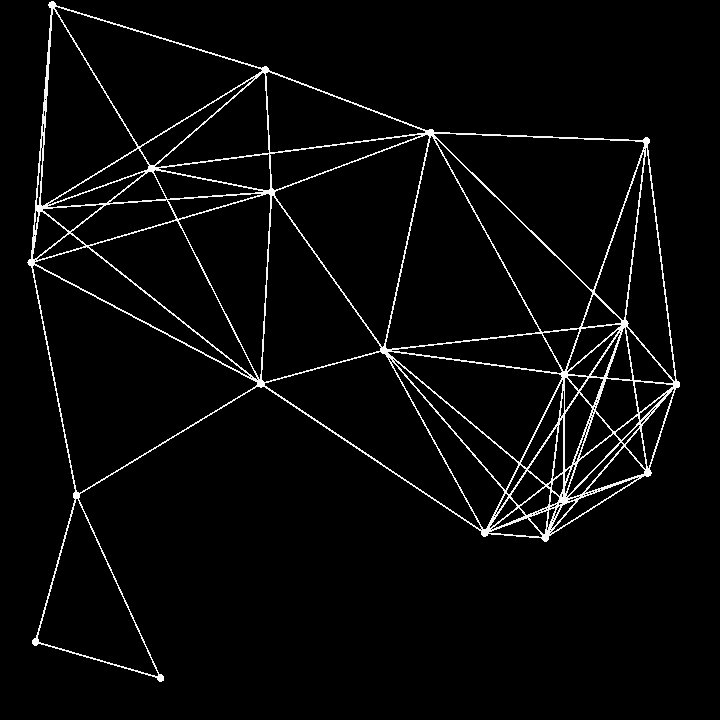
\includegraphics[width=\linewidth]{./images/slvo-0.png}}
            \end{minipage}
            \hspace{\fill}
            \begin{minipage}{0.2\textwidth}
            \colorbox{gray}{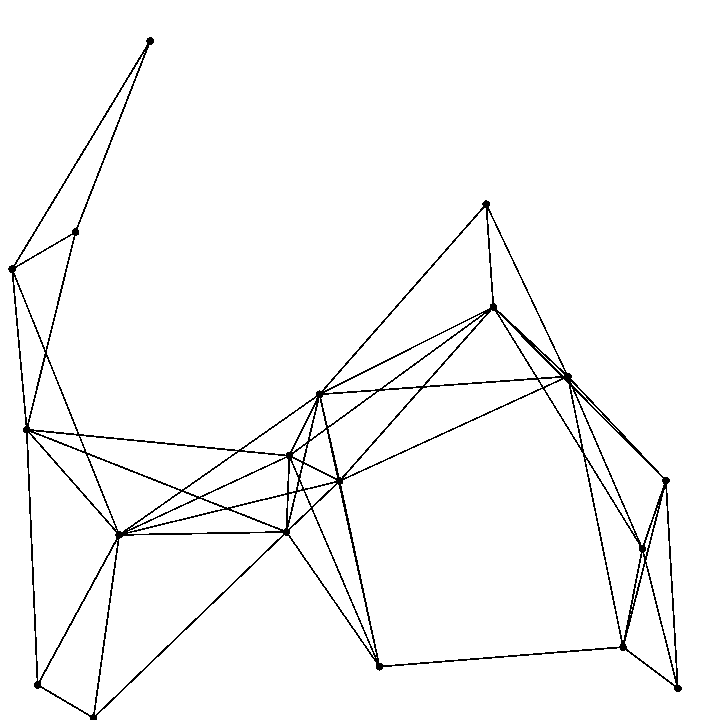
\includegraphics[width=\linewidth]{./images/slvo-1.png}}
            \end{minipage}
            \hspace{\fill}
            \begin{minipage}{0.2\textwidth}
            \colorbox{gray}{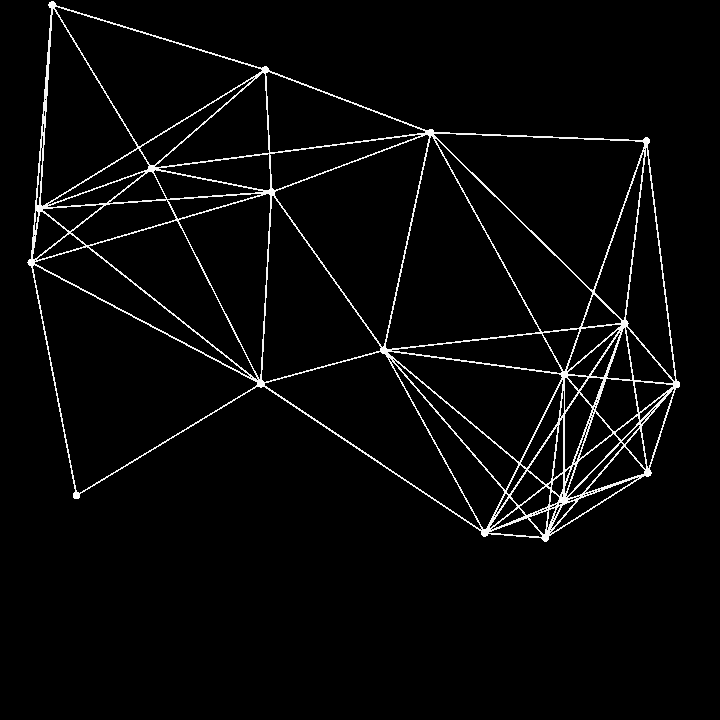
\includegraphics[width=\linewidth]{./images/slvo-2.png}}
            \end{minipage}
            \hspace{\fill}
            \begin{minipage}{0.2\textwidth}
            \colorbox{gray}{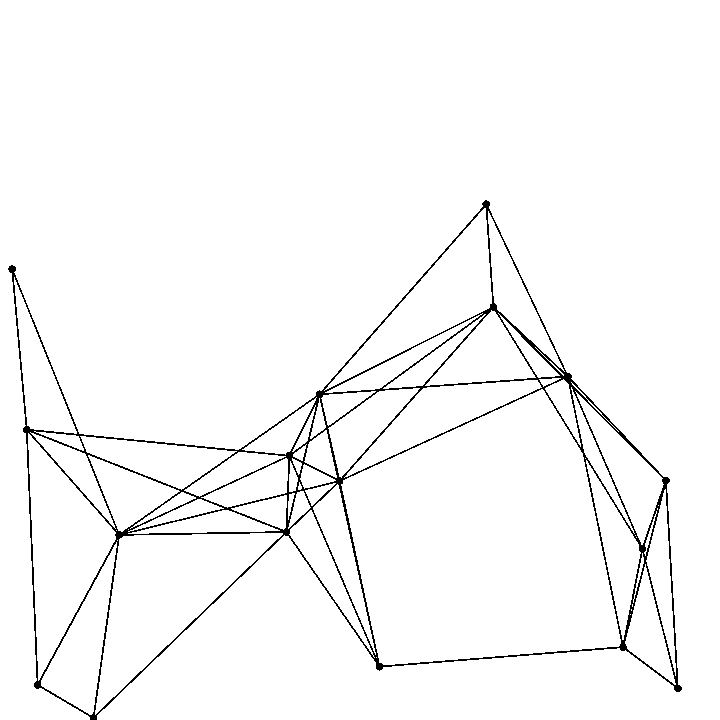
\includegraphics[width=\linewidth]{./images/slvo-3.png}}
            \end{minipage}
            \vskip 0.1in
            \begin{minipage}{0.2\textwidth}
            \colorbox{gray}{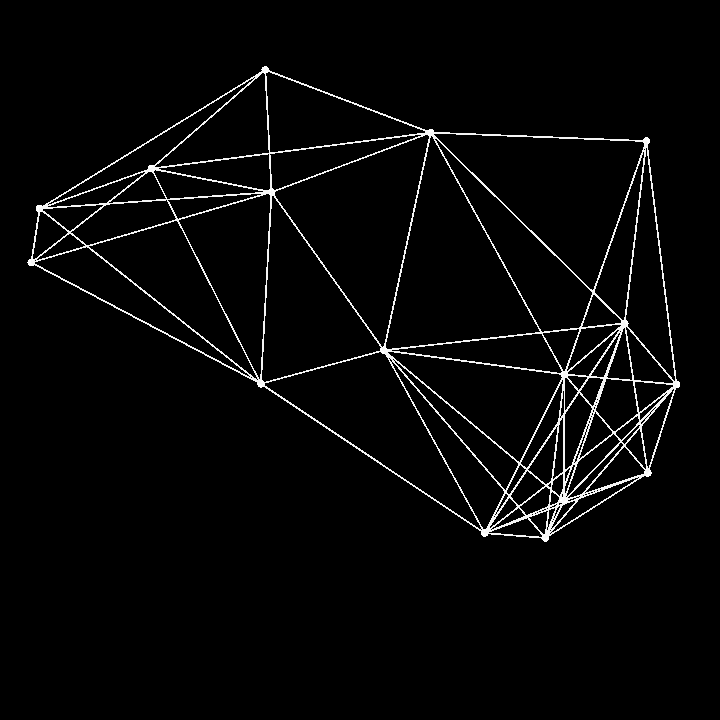
\includegraphics[width=\linewidth]{./images/slvo-4.png}}
            \end{minipage}
            \hspace{\fill}
            \begin{minipage}{0.2\textwidth}
            \colorbox{gray}{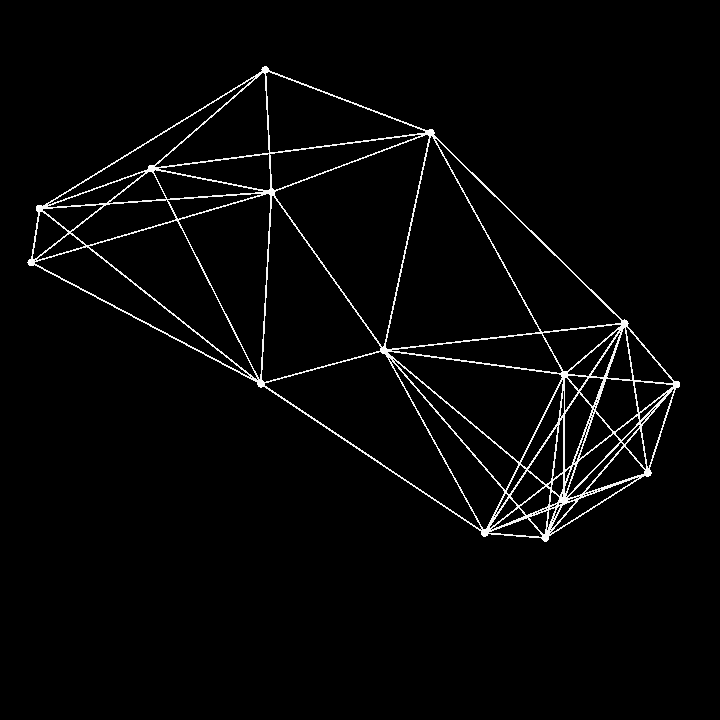
\includegraphics[width=\linewidth]{./images/slvo-5.png}}
            \end{minipage}
            \hspace{\fill}
            \begin{minipage}{0.2\textwidth}
            \colorbox{gray}{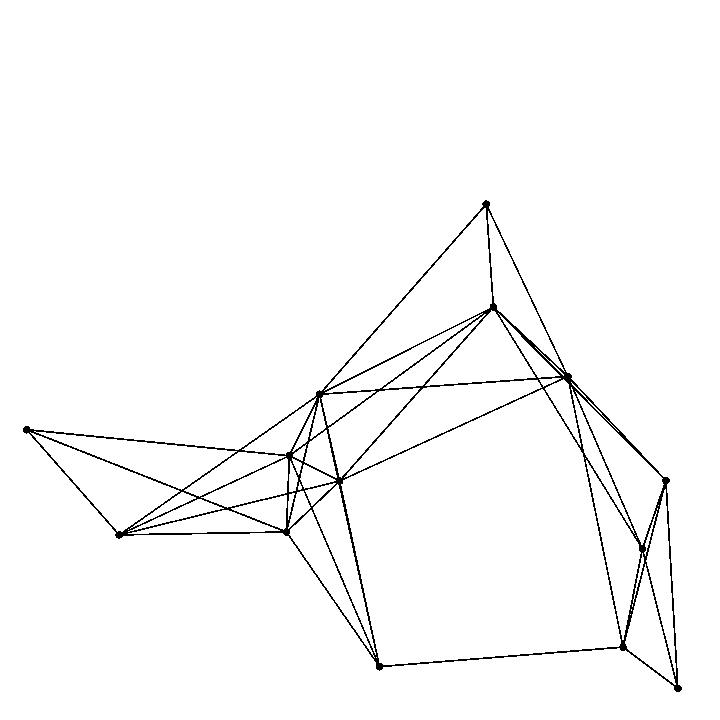
\includegraphics[width=\linewidth]{./images/slvo-6.png}}
            \end{minipage}
            \hspace{\fill}
            \begin{minipage}{0.2\textwidth}
            \colorbox{gray}{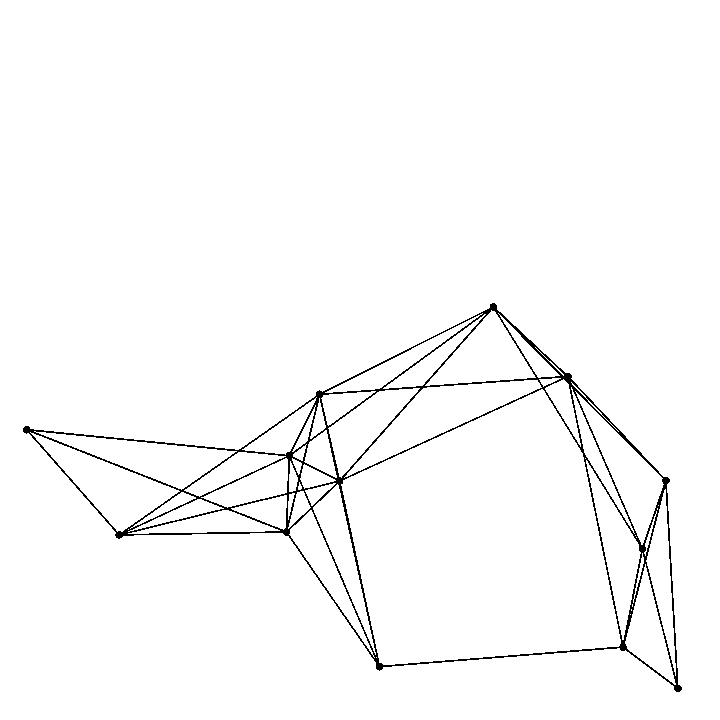
\includegraphics[width=\linewidth]{./images/slvo-7.png}}
            \end{minipage}
            \vskip 0.1in
            \begin{minipage}{0.2\textwidth}
            \colorbox{gray}{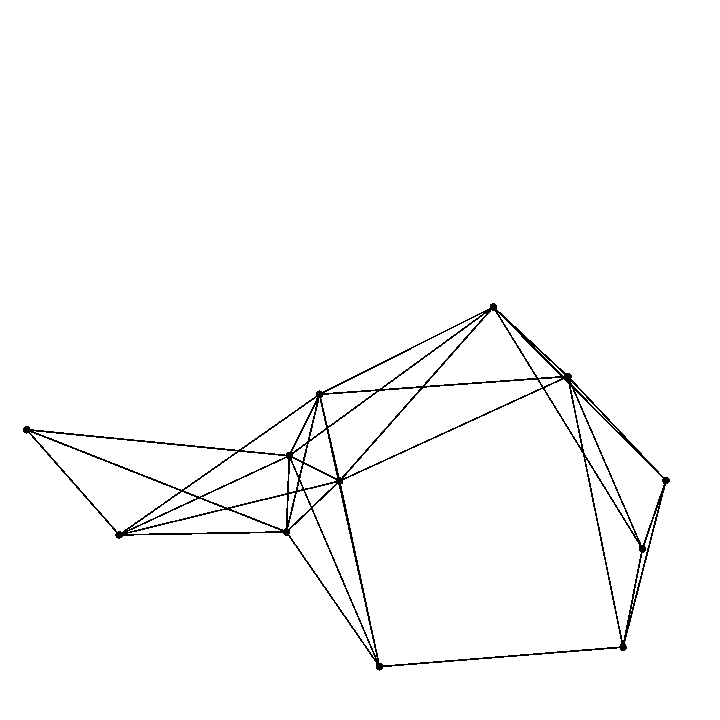
\includegraphics[width=\linewidth]{./images/slvo-8.png}}
            \end{minipage}
            \hspace{\fill}
            \begin{minipage}{0.2\textwidth}
            \colorbox{gray}{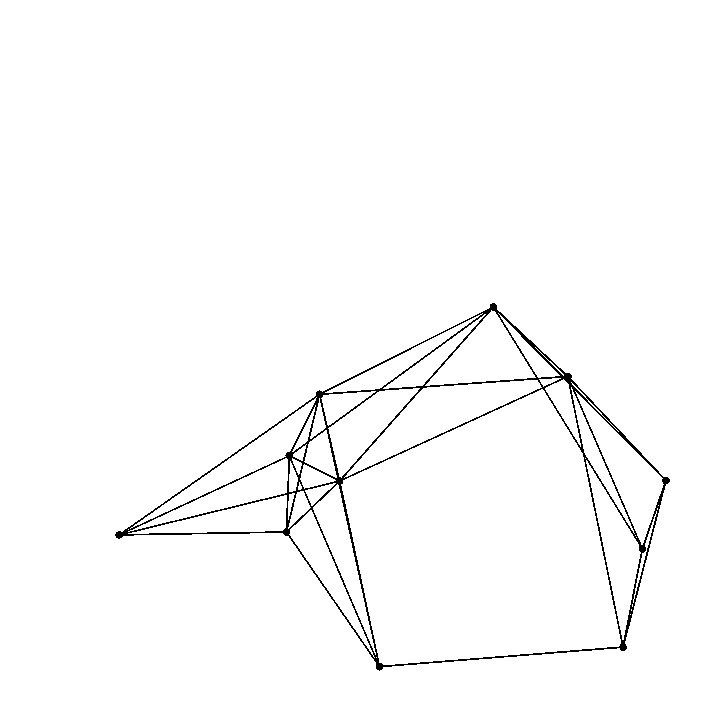
\includegraphics[width=\linewidth]{./images/slvo-9.png}}
            \end{minipage}
            \hspace{\fill}
            \begin{minipage}{0.2\textwidth}
            \colorbox{gray}{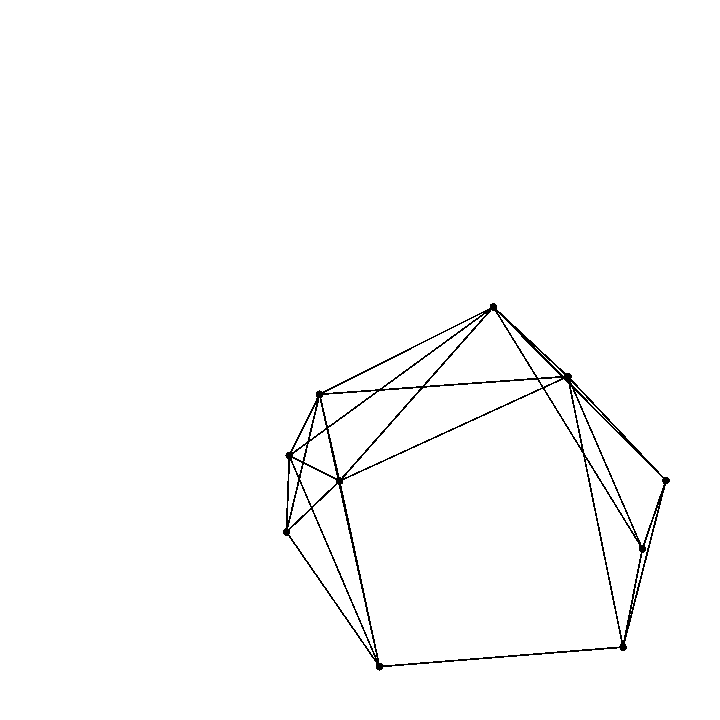
\includegraphics[width=\linewidth]{./images/slvo-10.png}}
            \end{minipage}
            \hspace{\fill}
            \begin{minipage}{0.2\textwidth}
            \colorbox{gray}{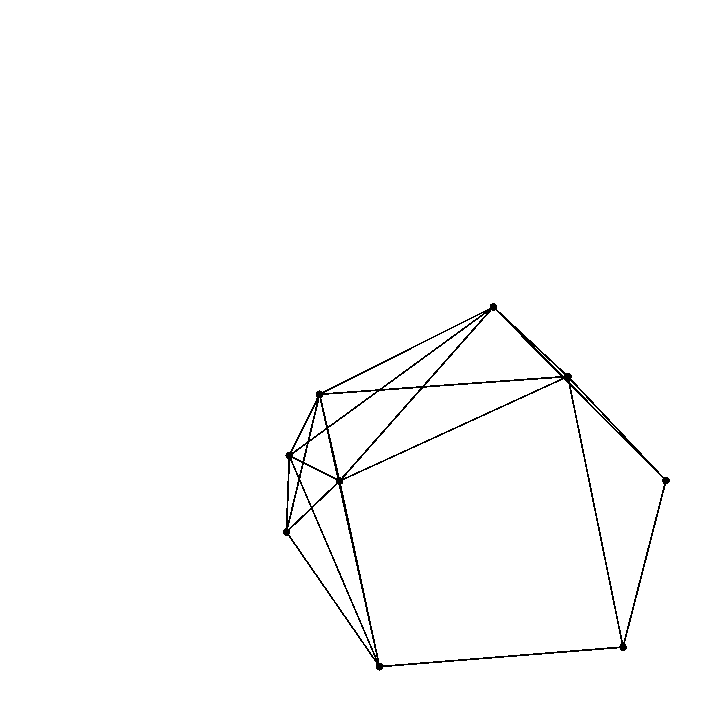
\includegraphics[width=\linewidth]{./images/slvo-11.png}}
            \end{minipage}
            \vskip 0.1in
            \begin{minipage}{0.2\textwidth}
            \colorbox{gray}{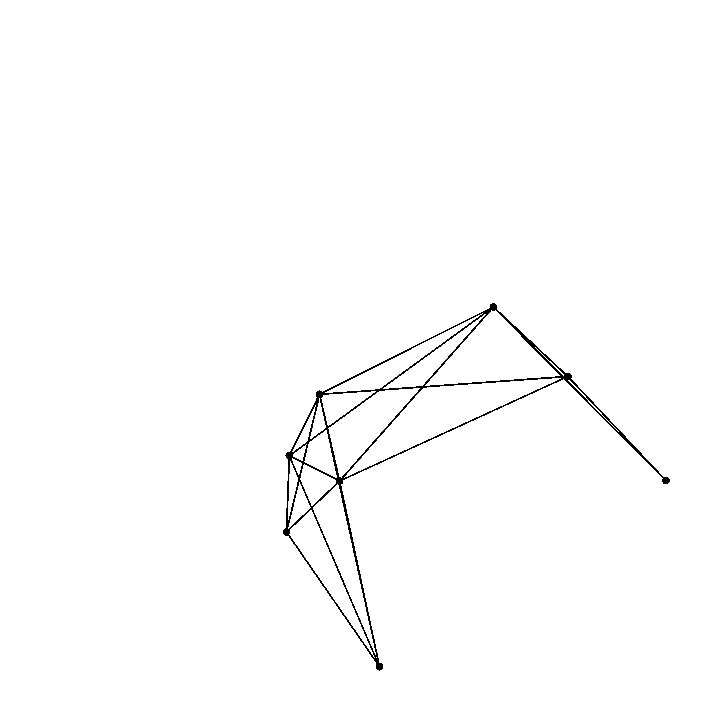
\includegraphics[width=\linewidth]{./images/slvo-12.png}}
            \end{minipage}
            \hspace{\fill}
            \begin{minipage}{0.2\textwidth}
            \colorbox{gray}{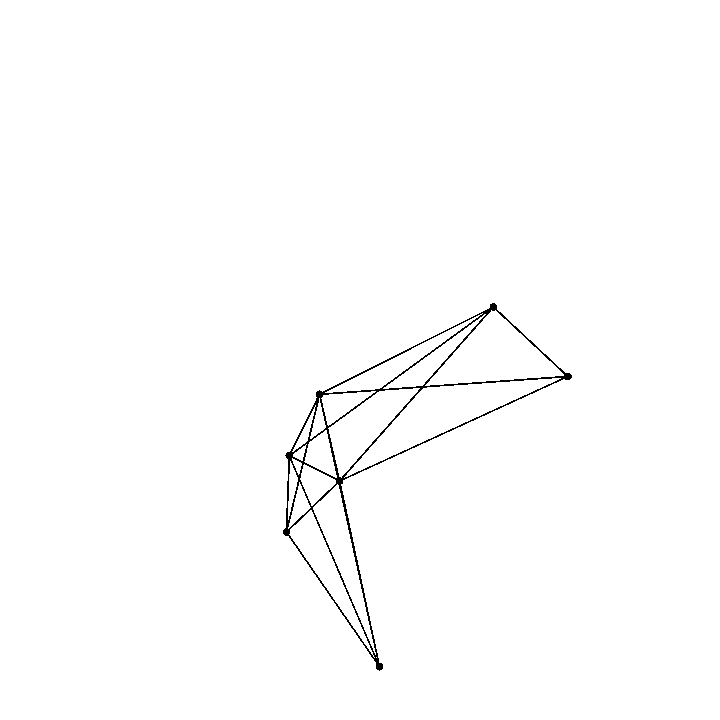
\includegraphics[width=\linewidth]{./images/slvo-13.png}}
            \end{minipage}
            \hspace{\fill}
            \begin{minipage}{0.2\textwidth}
            \colorbox{gray}{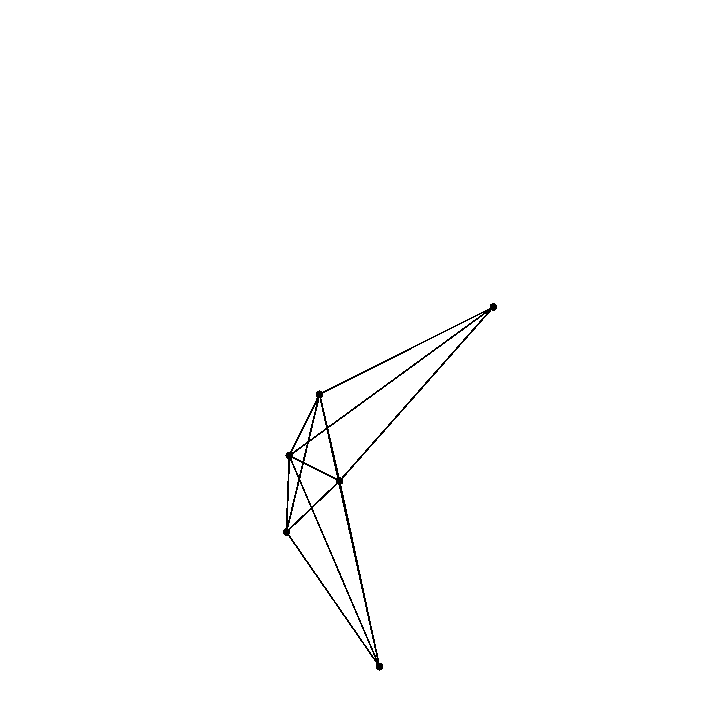
\includegraphics[width=\linewidth]{./images/slvo-14.png}}
            \end{minipage}
            \hspace{\fill}
            \begin{minipage}{0.2\textwidth}
            \colorbox{gray}{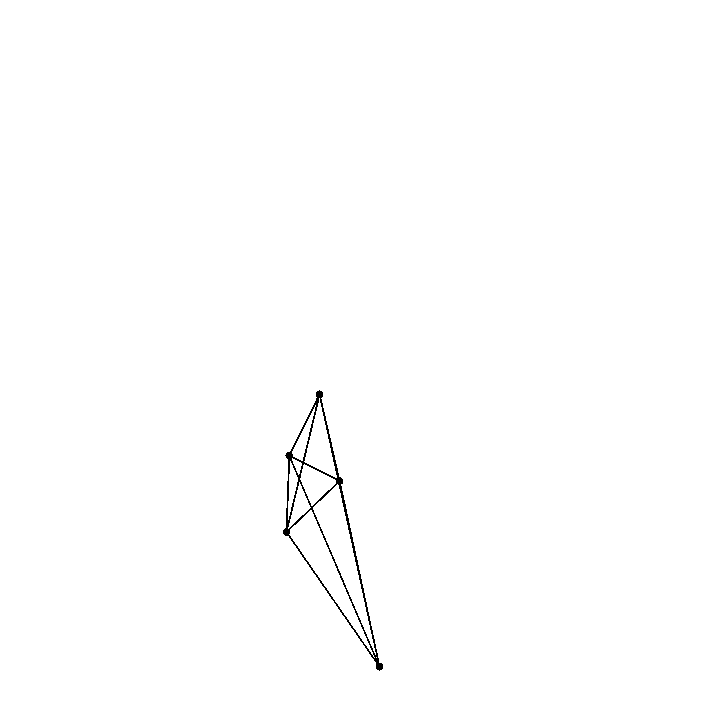
\includegraphics[width=\linewidth]{./images/slvo-15.png}}
            \end{minipage}
            \vskip 0.1in
            \begin{minipage}{0.2\textwidth}
            \colorbox{gray}{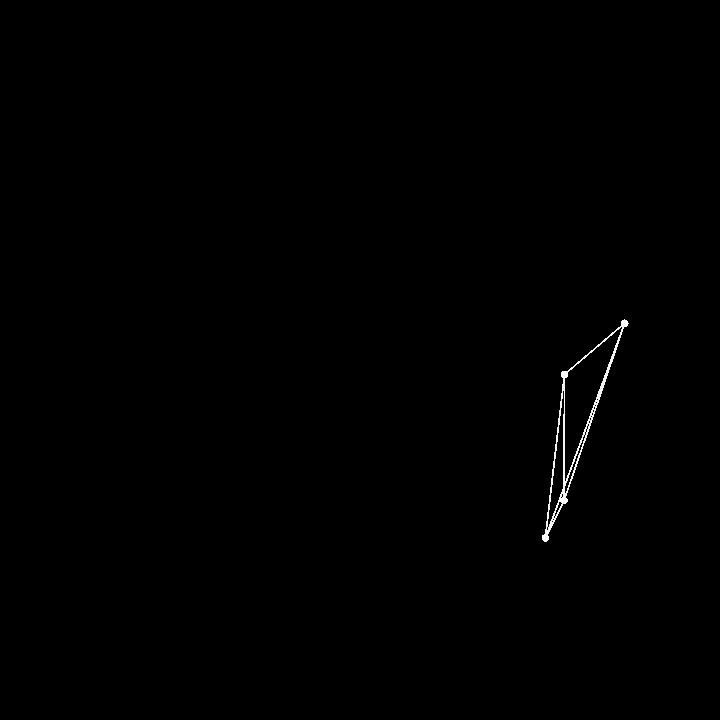
\includegraphics[width=\linewidth]{./images/slvo-16.png}}
            \end{minipage}
            \hspace{\fill}
            \begin{minipage}{0.2\textwidth}
            \colorbox{gray}{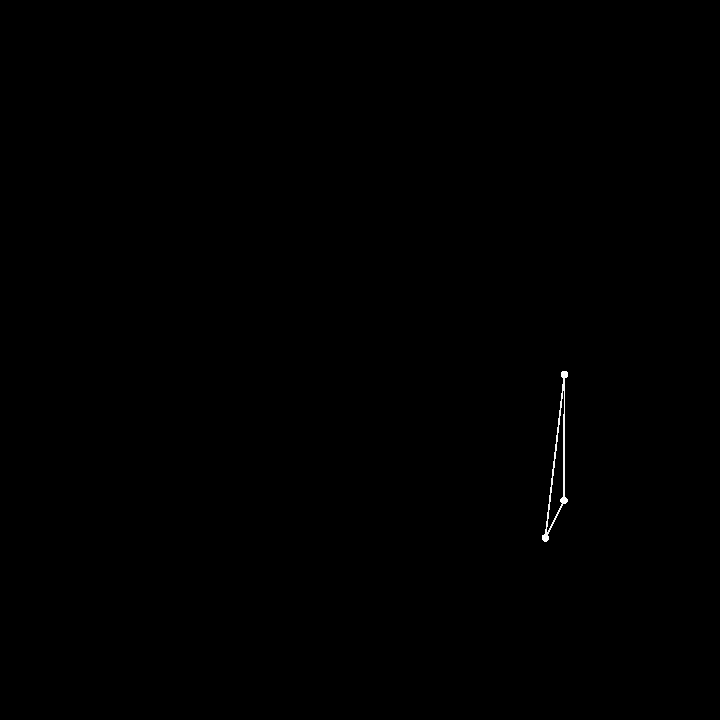
\includegraphics[width=\linewidth]{./images/slvo-17.png}}
            \end{minipage}
            \hspace{\fill}
            \begin{minipage}{0.2\textwidth}
            \colorbox{gray}{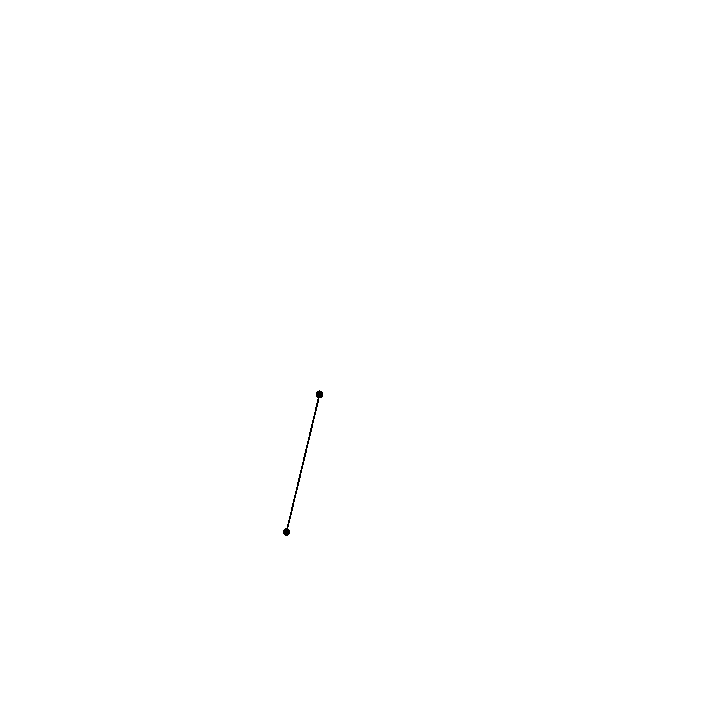
\includegraphics[width=\linewidth]{./images/slvo-18.png}}
            \end{minipage}
            \hspace{\fill}
            \begin{minipage}{0.2\textwidth}
            \colorbox{gray}{
\includegraphics[width=\linewidth]{./images/slvo-19.png}}
            \end{minipage}

            \caption{Smallest-last vertex ordering deletion process}
            \label{slvodel}
        \end{figure}

        \begin{figure}
            \begin{minipage}{0.2\textwidth}
            \colorbox{gray}{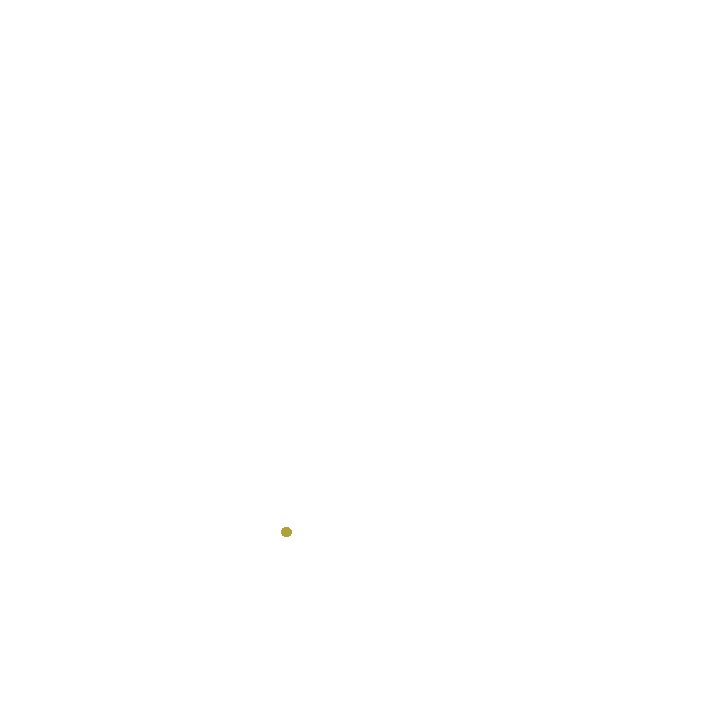
\includegraphics[width=\linewidth]{./images/color-1.png}}
            \end{minipage}
            \hspace{\fill}
            \begin{minipage}{0.2\textwidth}
            \colorbox{gray}{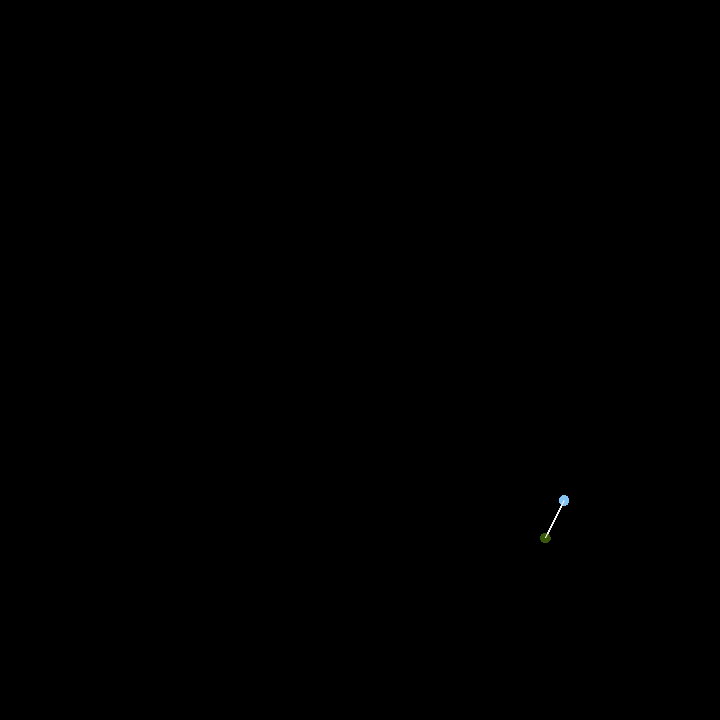
\includegraphics[width=\linewidth]{./images/color-2.png}}
            \end{minipage}
            \hspace{\fill}
            \begin{minipage}{0.2\textwidth}
            \colorbox{gray}{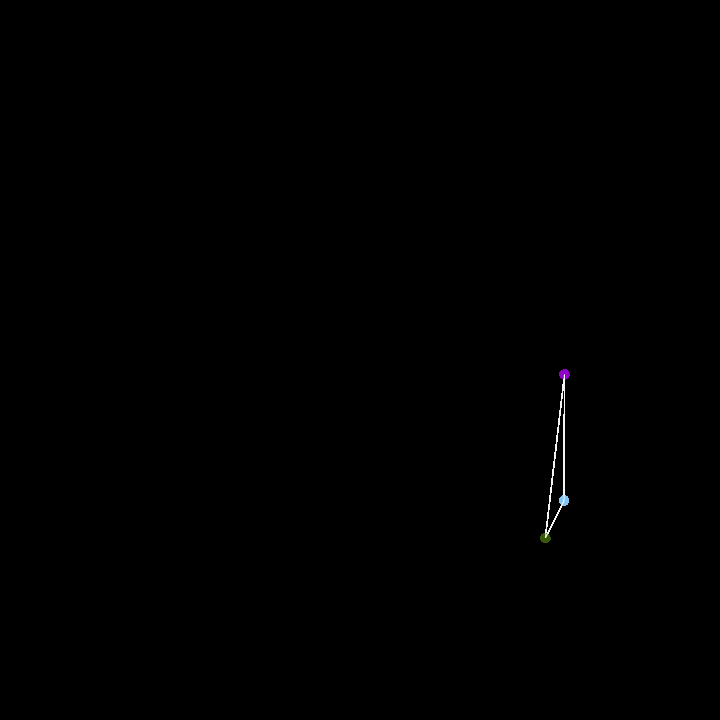
\includegraphics[width=\linewidth]{./images/color-3.png}}
            \end{minipage}
            \hspace{\fill}
            \begin{minipage}{0.2\textwidth}
            \colorbox{gray}{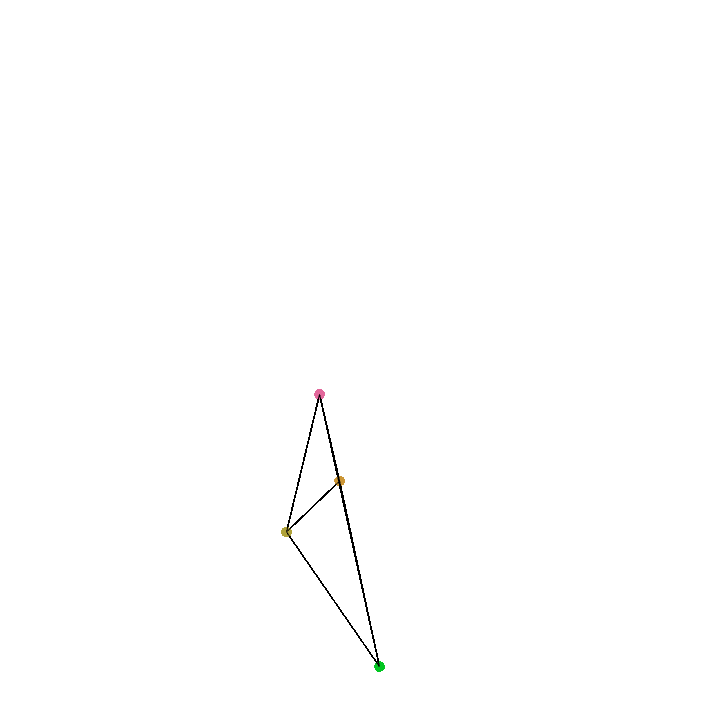
\includegraphics[width=\linewidth]{./images/color-4.png}}
            \end{minipage}
            \vskip 0.1in
            \begin{minipage}{0.2\textwidth}
            \colorbox{gray}{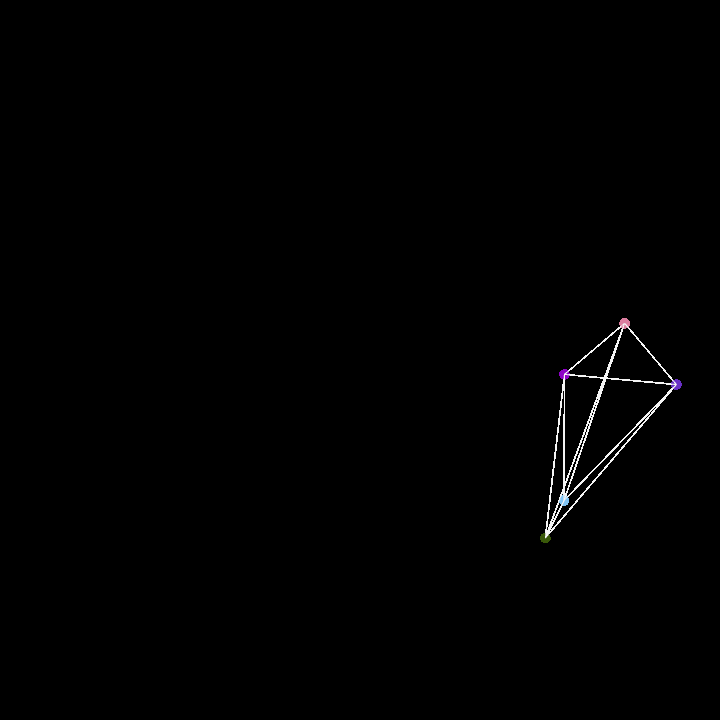
\includegraphics[width=\linewidth]{./images/color-5.png}}
            \end{minipage}
            \hspace{\fill}
            \begin{minipage}{0.2\textwidth}
            \colorbox{gray}{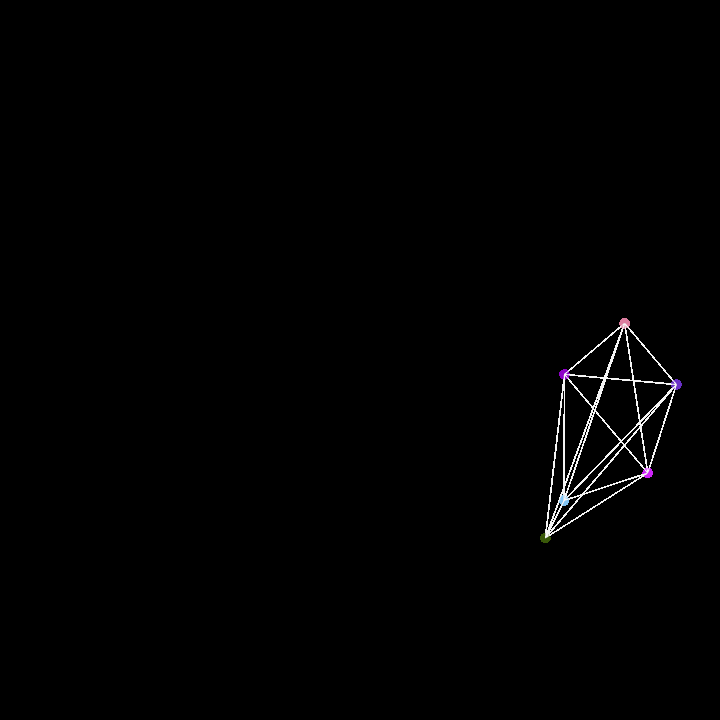
\includegraphics[width=\linewidth]{./images/color-6.png}}
            \end{minipage}
            \hspace{\fill}
            \begin{minipage}{0.2\textwidth}
            \colorbox{gray}{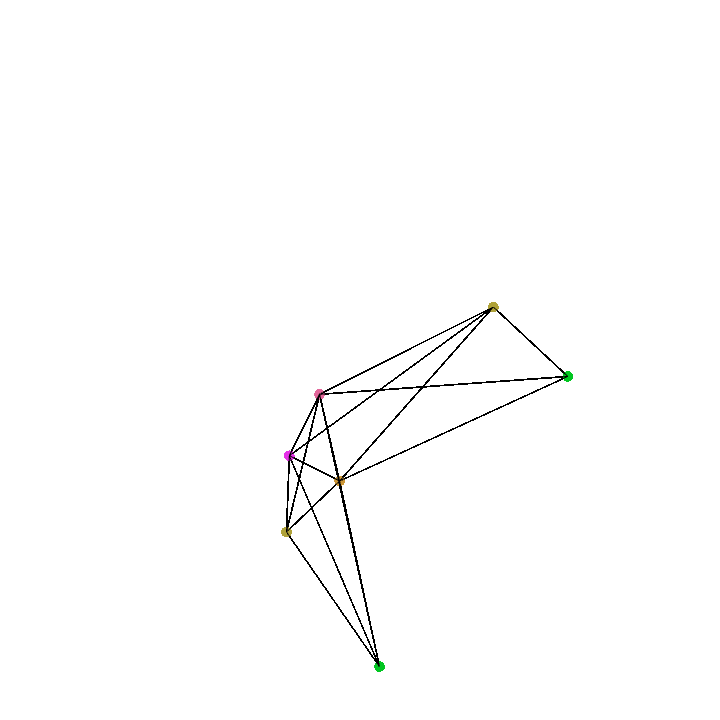
\includegraphics[width=\linewidth]{./images/color-7.png}}
            \end{minipage}
            \hspace{\fill}
            \begin{minipage}{0.2\textwidth}
            \colorbox{gray}{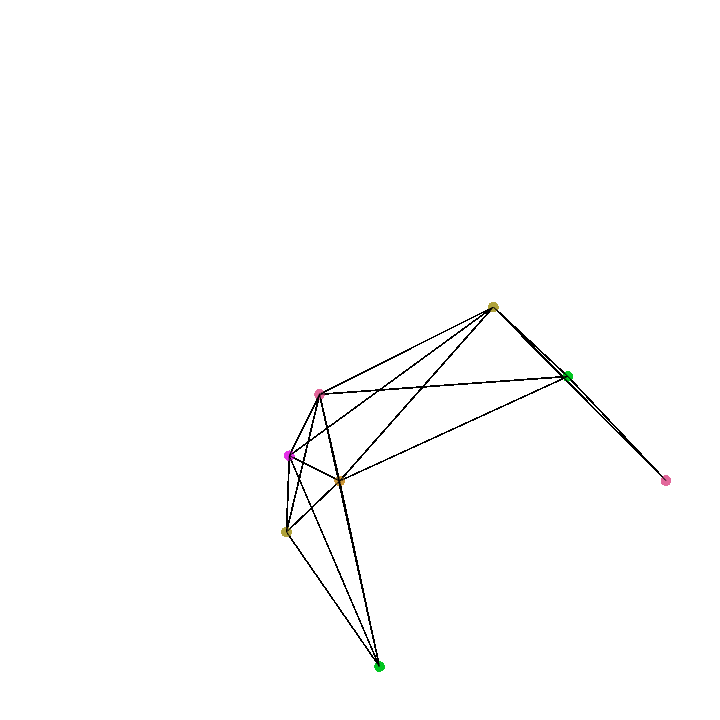
\includegraphics[width=\linewidth]{./images/color-8.png}}
            \end{minipage}
            \vskip 0.1in
            \begin{minipage}{0.2\textwidth}
            \colorbox{gray}{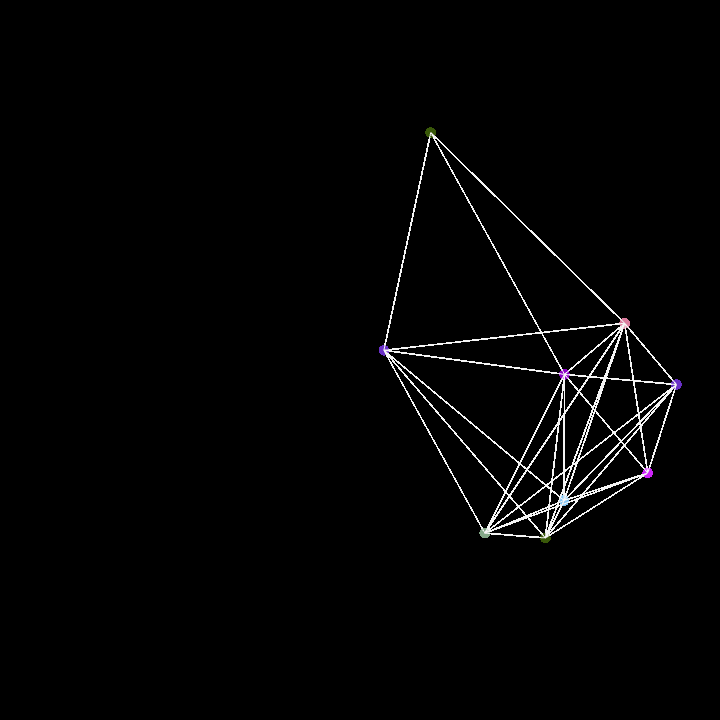
\includegraphics[width=\linewidth]{./images/color-9.png}}
            \end{minipage}
            \hspace{\fill}
            \begin{minipage}{0.2\textwidth}
            \colorbox{gray}{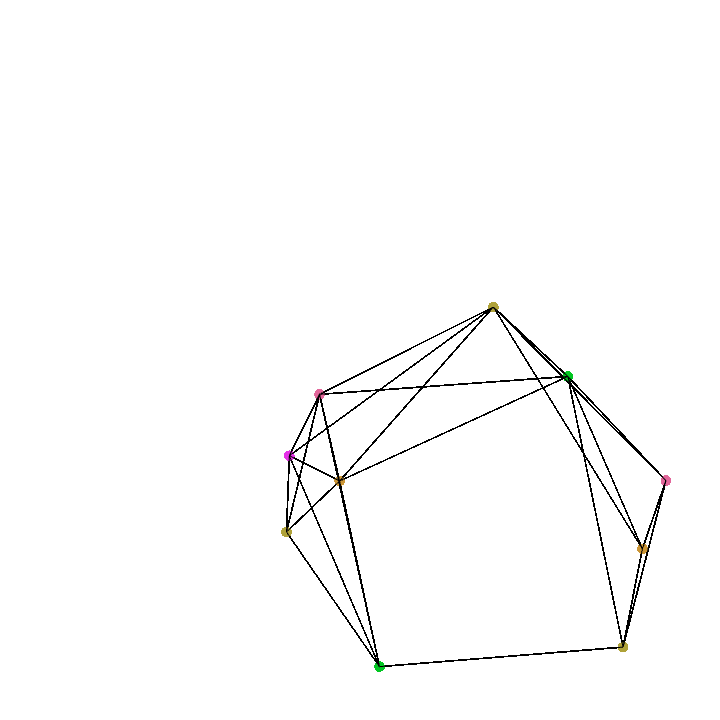
\includegraphics[width=\linewidth]{./images/color-10.png}}
            \end{minipage}
            \hspace{\fill}
            \begin{minipage}{0.2\textwidth}
            \colorbox{gray}{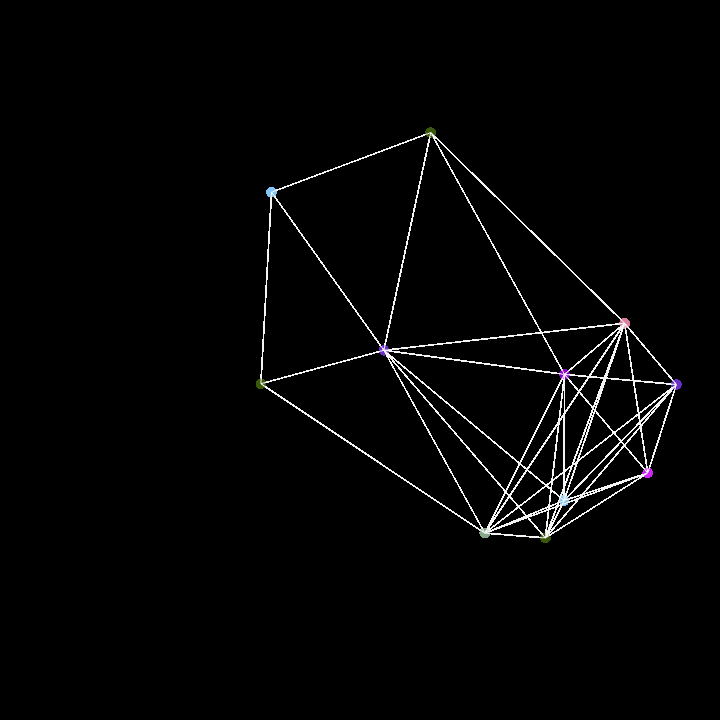
\includegraphics[width=\linewidth]{./images/color-11.png}}
            \end{minipage}
            \hspace{\fill}
            \begin{minipage}{0.2\textwidth}
            \colorbox{gray}{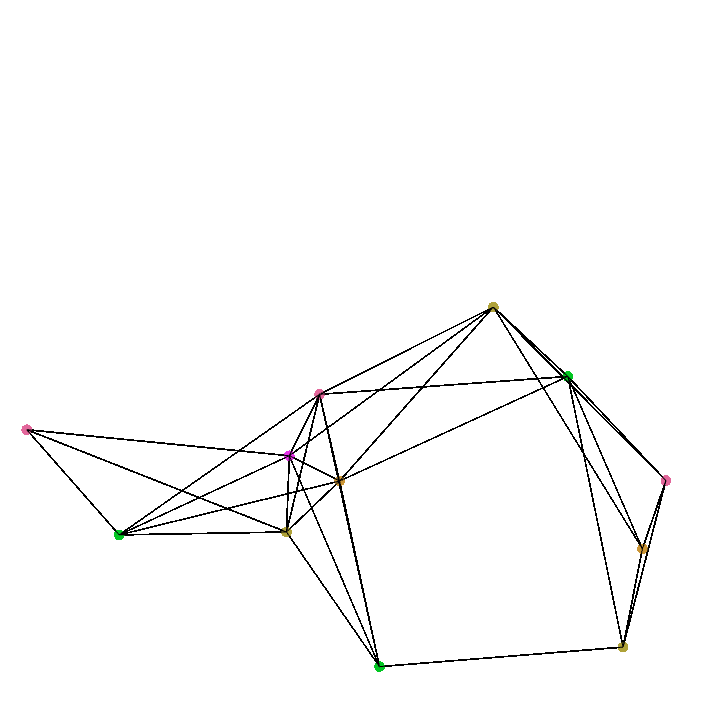
\includegraphics[width=\linewidth]{./images/color-12.png}}
            \end{minipage}
            \vskip 0.1in
            \begin{minipage}{0.2\textwidth}
            \colorbox{gray}{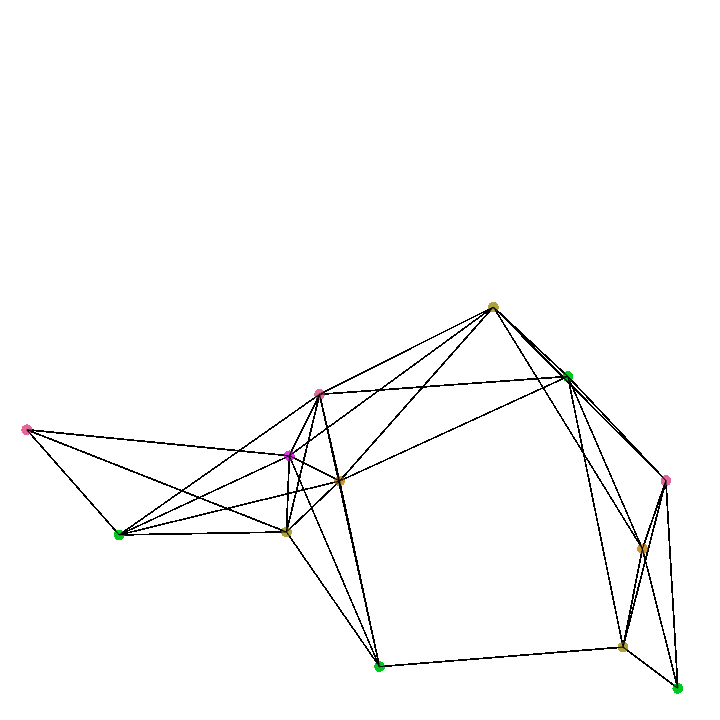
\includegraphics[width=\linewidth]{./images/color-13.png}}
            \end{minipage}
            \hspace{\fill}
            \begin{minipage}{0.2\textwidth}
            \colorbox{gray}{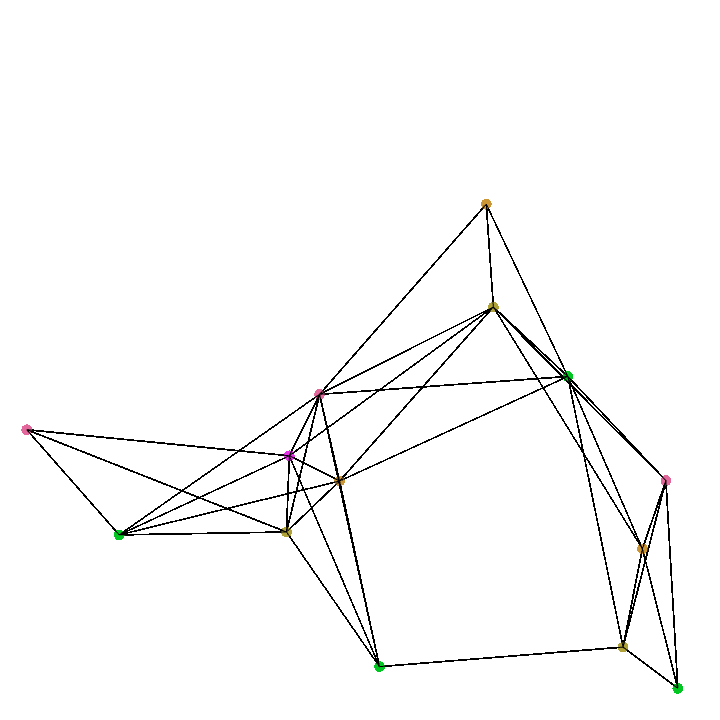
\includegraphics[width=\linewidth]{./images/color-14.png}}
            \end{minipage}
            \hspace{\fill}
            \begin{minipage}{0.2\textwidth}
            \colorbox{gray}{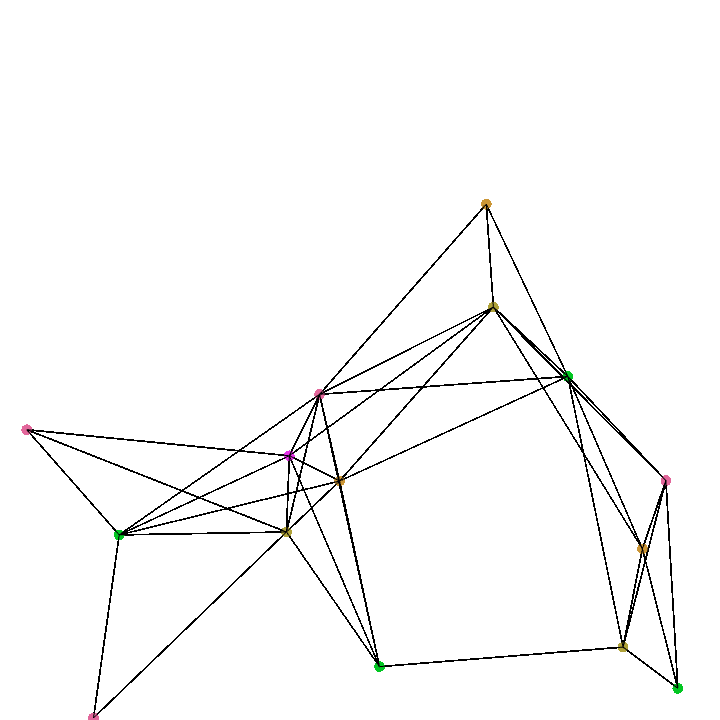
\includegraphics[width=\linewidth]{./images/color-15.png}}
            \end{minipage}
            \hspace{\fill}
            \begin{minipage}{0.2\textwidth}
            \colorbox{gray}{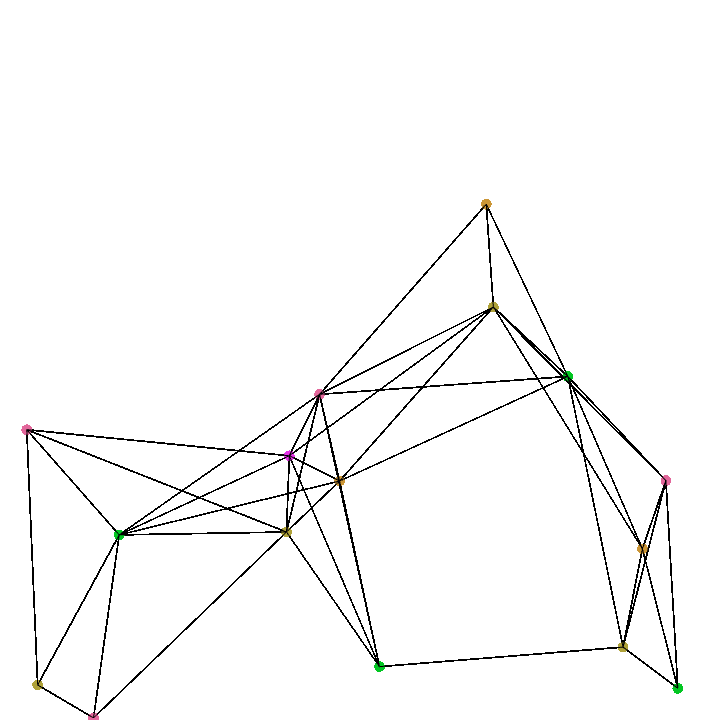
\includegraphics[width=\linewidth]{./images/color-16.png}}
            \end{minipage}
            \vskip 0.1in
            \begin{minipage}{0.2\textwidth}
            \colorbox{gray}{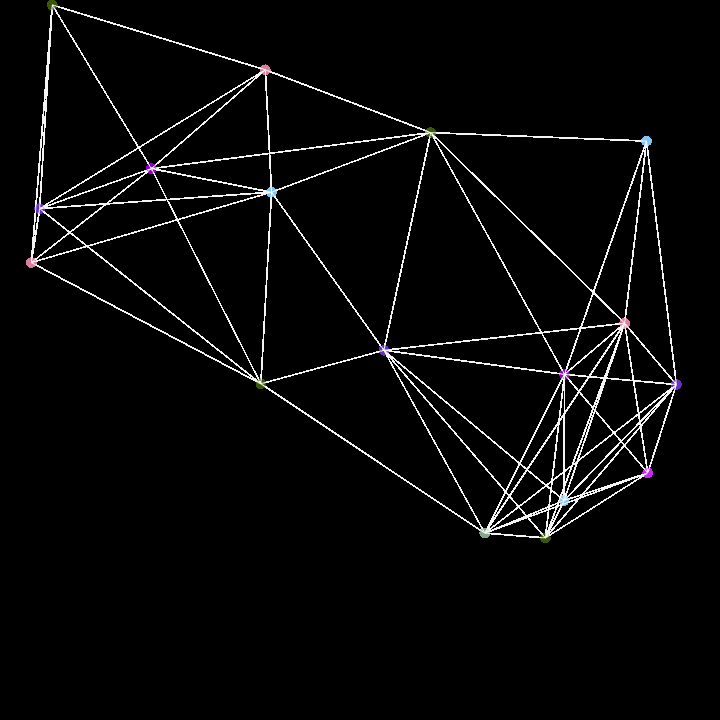
\includegraphics[width=\linewidth]{./images/color-17.png}}
            \end{minipage}
            \hspace{\fill}
            \begin{minipage}{0.2\textwidth}
            \colorbox{gray}{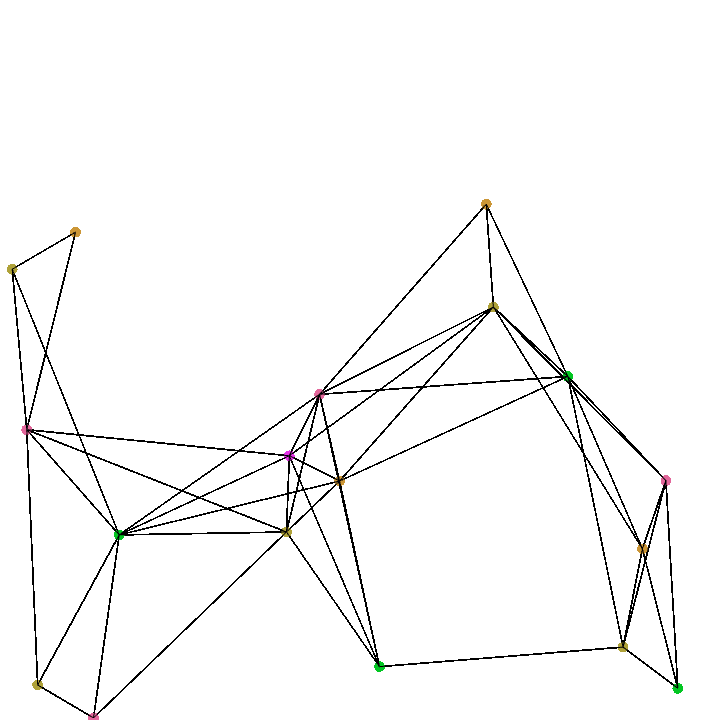
\includegraphics[width=\linewidth]{./images/color-18.png}}
            \end{minipage}
            \hspace{\fill}
            \begin{minipage}{0.2\textwidth}
            \colorbox{gray}{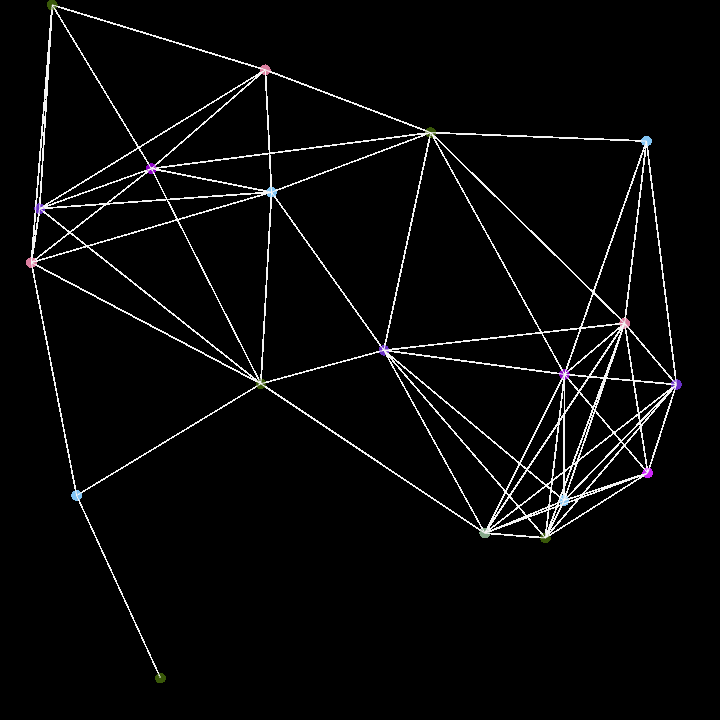
\includegraphics[width=\linewidth]{./images/color-19.png}}
            \end{minipage}
            \hspace{\fill}
            \begin{minipage}{0.2\textwidth}
            \colorbox{gray}{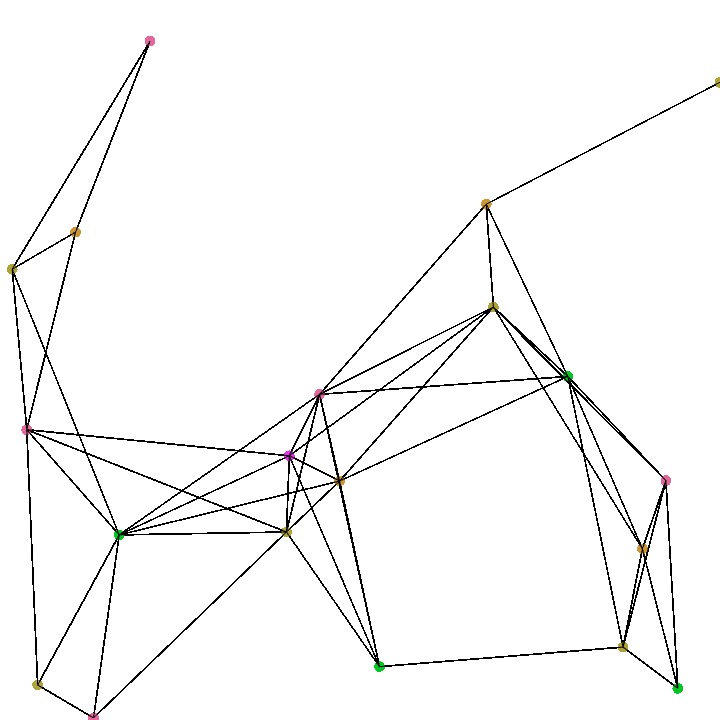
\includegraphics[width=\linewidth]{./images/color-20.png}}
            \end{minipage}

            \caption{Smallest-last vertex ordering coloring process}
            \label{slvocolor}
        \end{figure}

        \begin{figure}
            \begin{minipage}{0.45\textwidth}
            \colorbox{gray}{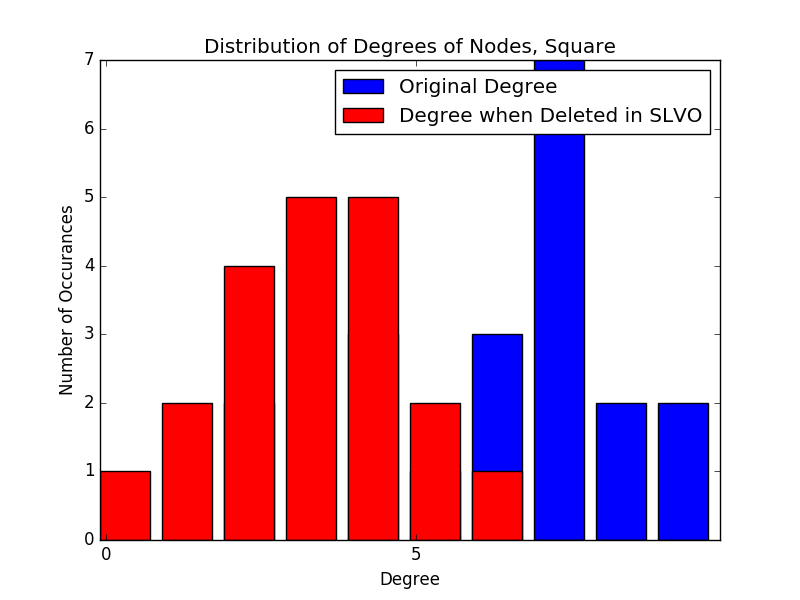
\includegraphics[width=\linewidth]{./graphs/hist_deg_del_wt.png}}
            \end{minipage}
            \hspace{\fill}
            \begin{minipage}{0.45\textwidth}
            \colorbox{gray}{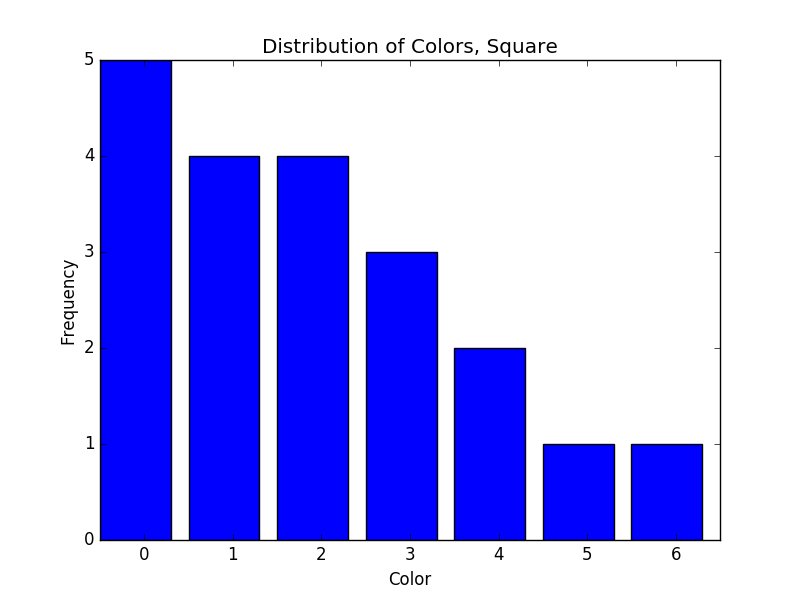
\includegraphics[width=\linewidth]{./graphs/hist_colors_wt.png}}
            \end{minipage}

            \caption{Distribution of degree when deleted and color set size for the 20 node walkthrough}
            \label{histwt}
        \end{figure}

        \subsubsection{Backbone Determination}
        Implementing backbone determination requires implementing all of the algorithms needed to create the bipartite subgraphs, remove unwanted nodes, and find the major components. Pairing the independent color sets is the most straightforward algorithm to implement. First, a list of four sets is created to hold the four largest independent color sets. Since the largest color sets will be the first four colors used in the greedy graph coloring implementation, all of the nodes are iterated over and each one is checked to see if its color is less than four. If that is the case, it is added to the independent set at that index in the initial list. Then, the list of independent sets is iterated over and each set is unioned with each remaining set in the list to get all of the combinations of the independent sets. The Python set union operation iterates over all of the items in each set and adds them to a result set. Since this is called three times on each independent set, and because the nodes needed to be iterated over once to place the nodes in their color sets, the total runtime for this implementation is $O(4|V|)$. The total space used by this algorithm is $O(4|V|)$, because four copies are made of each independent set. However, one of each of these copies is removed when the function returns the combinations.
        \par
        Next, the independent color set pairings need to be cleaned. This is a multi-step process that starts with the removal of tails from the bipartites. Like stated earlier, the algorithm to remove tails is similar to the smallest-last vertex ordering algorithm with an early stopping condition for when the bucket for degree 1 is empty. First, some accessory data structures are initialized to save information about the representation of the graph while nodes are deleted. The buckets are initialized as empty sets. The total number of buckets needed is equal to the degree of the node with the max degree. A map is needed to relate each node to its bucket, which is created by iterating over all of the nodes in the bipartite, and counting the number of edges it shares with other nodes in the bipartite. Then, the nodes are iterated over again and placed in their buckets. At this point, the total space used is $\Theta(2|V|)$ and the time used is $\Theta(2|V| + 2|E|)$.
        \par
        At this point, the smallest-last vertex algorithm is run until the sets for degree zero and one are empty. Each iteration of the algorithm, all of the nodes in the degree zero and degree one sets are put in a list of nodes to remove. Both sets are checked so that any nodes in the graph that are not connected to a component are removed. These nodes are then iterated over and each edge it shares with a node in the bipartite is checked to see if the neighbor needs to be moved down a bucket. Once all neighbors have been moved down, the node is removed from the bipartite subgraph. This runs in similar time as smallest-last vertex ordering, $\Theta(2|V| + 2|E|)$. The only additional space needed by the algorithm is the space needed to hold the list of nodes in the first two buckets, however, once the nodes have been copied into the list, the buckets they were in are cleared. Regardless, thin can use $O(|V|)$ in the worst case. All together, tail removal takes $O(3|V|)$ space and $\Theta(4|V| + 4|E|)$ time.
        \par
        The next part of the cleaning is selecting the major component, which is implemented using breadth-first search. Before starting BFS, some setup is needed. First, the bipartite is copied into a local list for iteration. Then, two dictionaries are created for indexing from the local list of bipartite nodes to the master list of nodes. Next, a list of integers is created for keeping track of which nodes have been visited during BFS. At this point, $O(4|V|)$ space has been used. Then, BFS starts and runs until every node has been visited. While nodes have not been visited, the first unvisited node is selected to be the root of the search tree. This root is put in the queue, added as the first item in a set to a list of sets representing the components in the graph, and the visit time is set to 1. Then, while the queue is not empty, an item is popped and all of its edges are checked to see if they have already been visited. Each one that has not been visited is pushed into the queue, market as visited, added to the set representing the current component being searched, and the visit time is incremented. Once the queue is empty, the final visit time is saved as the number of nodes in the component. After all nodes have been visited, all that is needed is to return the component with the largest number of visits and the major component has been determined. This implementation of BFS requires $\Theta(|V| + 2|E|)$ time and $O(2|V|)$ space because the nodes are copied into their respective component sets, and the queue could grow to hold all nodes in the graph in the worst case.
        \par
        The last step in preparing the backbones is to remove all of the bridges and minor blocks. Bridge removal uses depth-first search, however, some other data is needed to keep track of the visit time for nodes (tin) and the visit time of their ancestors (fup) in the DFS tree. First, a local copy of the bipartite is created to iterate over, and, similar to BFS, two dictionaries are created for indexing between the local list of nodes and the master list of nodes. A list is created to keep track of whether nodes have been visited or not, the visit time of the DFS algorithm at the node, and the minimum visit time of a nodes decendents. All of these data structures together require $\Theta(6|V|)$ space and can be created in $\Theta(6|V|)$ time. Now, DFS can run until all of the nodes have been visited. The first node that hasn't been visited is selected as the root of the search tree for DFS. Each edge this node shares with another node in the major component is iterated over. Fup for the current node is calculated for each of the neighbor nodes that has not been visited as the mimimum of fup for the current node and tin of the current edge. If the neighbor hasn't been visited, DFS is called recursively on the edge to search it. Once the search returns, fup for the current node is calculated as the minimum of fup for the current node and fup for the current edge. There is now enough information to determine if the current edge is a bridge. If fup for the current edge is greater than tin for the current node, then the neighbor must not have another path to any of the ancestors of the current node, so it is a bridge and the current nodes are saved to a list of bridges. DFS itself runs in $\Theta(|V| + 2|E|)$ time and uses $O(2|E|)$ space in the worst case which would be that all nodes in the graph are part of a bridge (however, this would never happen because tails have already been removed).
        \par
        The final step of bridge removal is to use the list of nodes that are part of the bridges to determine the major component with the bridges removed. BFS is suitable for this because it is already implemented to return the major component of a graph. In order to make BFS skip the bridge nodes, each time an edge is visited that has both nodes in the set of bridge nodes, continue is called to skip the rest of the iteration. This will prevent pushing that neighbor to the queue and will disconnect those components. BFS will then proceed and return the major component. All together, bridge removal uses $O(8|V| + 2|E|)$ space and runs in $\Theta(8|V| + 4|E|)$ time.
        \par
        At this point, six potential backbones have been determined from the original six bipartite subgraphs. Now, the two largest backbones need to be determined. These are the backbones with the largest size, or the highest number of edges. To find the two largest backbones, two parallel lists are created that each have two elements. The first list is for the sizes of the backbones, and the second is for the backbones themselves. For each backbone, the size is calculated by iterating over all the nodes in the backbone and summing the number of edges each node shares with another node in the backbone. Because the backbones are represented as a set, it takes constant time to see if a node is in the backbone. Once the size has been calculated for a backbone, it is checked to see if it is larger than the saved backbone with the minimum size. If this is the case, it replaces that backbone in the list of results and its size is saved. This requires $\Theta(|V| + 2|E|)$ time for each backbone. After the two largest backbones have been determined, some metadata is calculated about them and returned as a parallel array to the list of backbones. This meta data is the order and size of each backbone, which is not dependent on the size of the backbones.
        \par
        Finally, the domination of the two largest backbones needs to be calculated. This is done by initializing a search space with all of the nodes in the master list of nodes that are not in the backbone. This search space is then iterated over, and each edge is checked to see if the neighboring node is in the backbone. If a node does share an edge with the backbone, it is removed from the search space. Also, once it has been found that the current node shares an edge with a backbone node, the rest of the edges for the current node can be skipped. At the end of this, the search space will have all nodes that do not share an edge with a backbone node. It is then easy to calculate the domination of the backbone by subtracting this number from the total number of nodes and dividing by the total number of nodes. This runs in $\Theta(|V| + |E|)$ time and requires $\Theta(|V|)$ space to initialize the search space.
        \par
        If the topology is a sphere, the number of faces of the backbone can be calculated using Euler's Polyhedral Formula. This formula operates under the assumption that a graph is connected and can be represented in planar form. The first is guaranteed because the backbone is the major connected component found in a bipartite subgraph. The second is true because the nodes comprising the backbone can be projected onto a plane and there will be no overlapping edges because the edges do not overlap in the original representation. Therefore, the number of faces can be calculated in constant time using the meta data of the backbone generated earlier.
        \par
        To illustrate this further, the above walkthrough is extended to include the backbone determination stages based on the two largest color sets. These stages are given in Figure \ref{wtbackbone}. With the selected color sets, removing the tails is sufficient for creating the backbone. The other steps yield the same graph, but are necessary for higher-order graphs. It can be seen that the backbone is a planar graph because it can be embedded in a plane without any of the edges intersecting. The planarity of the backbone will be discussed further int he Verification section.

        \begin{figure}
            \begin{minipage}{0.3\textwidth}
            \colorbox{gray}{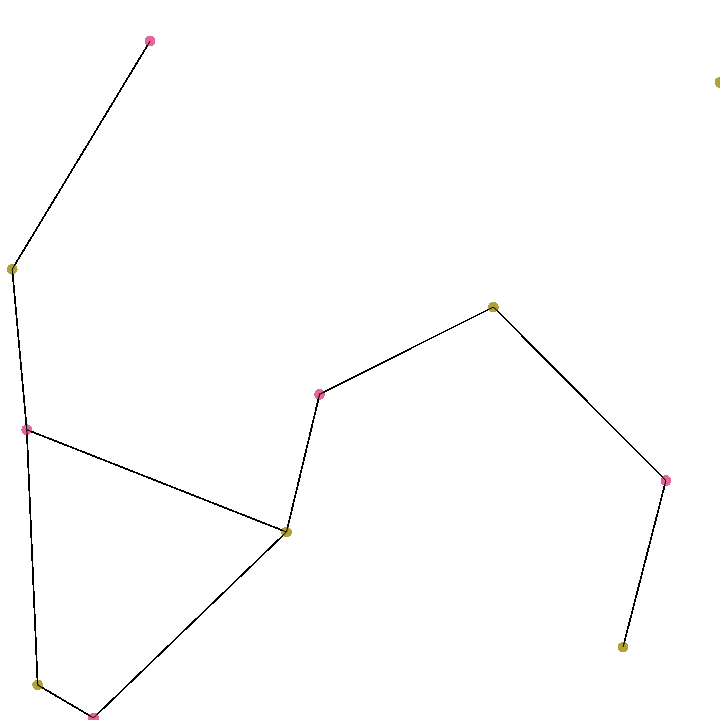
\includegraphics[width=\linewidth]{./images/bipartite-wt.png}}
            \end{minipage}
            \hspace{\fill}
            \begin{minipage}{0.3\textwidth}
            \colorbox{gray}{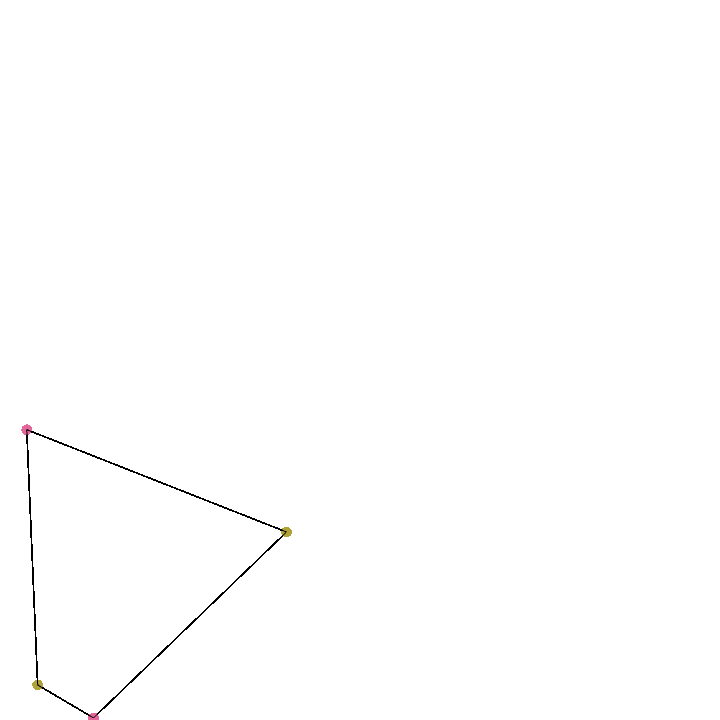
\includegraphics[width=\linewidth]{./images/no-tails-wt.png}}
            \end{minipage}
            \hspace{\fill}
            \begin{minipage}{0.3\textwidth}
            \colorbox{gray}{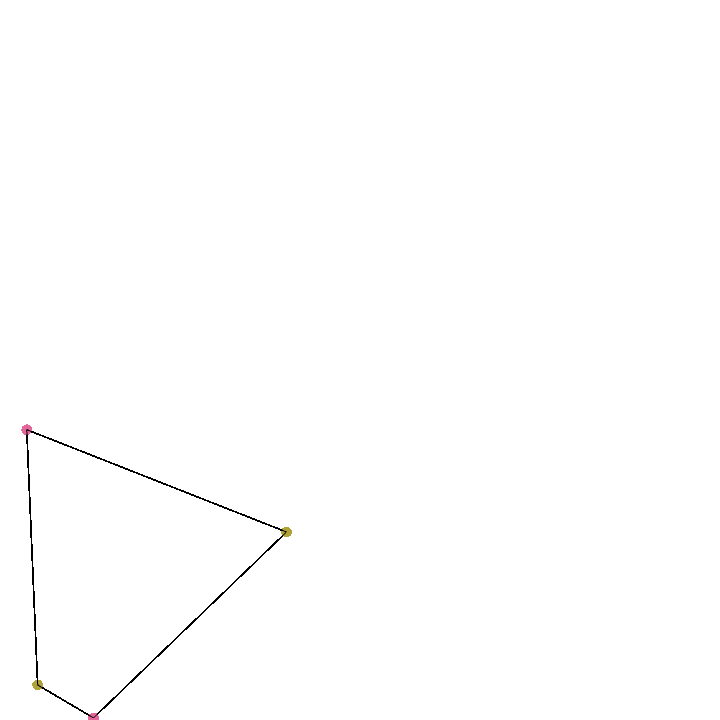
\includegraphics[width=\linewidth]{./images/major-comp-wt.png}}
            \end{minipage}
            \vskip 0.1in
            \begin{minipage}{0.3\textwidth}
            \colorbox{gray}{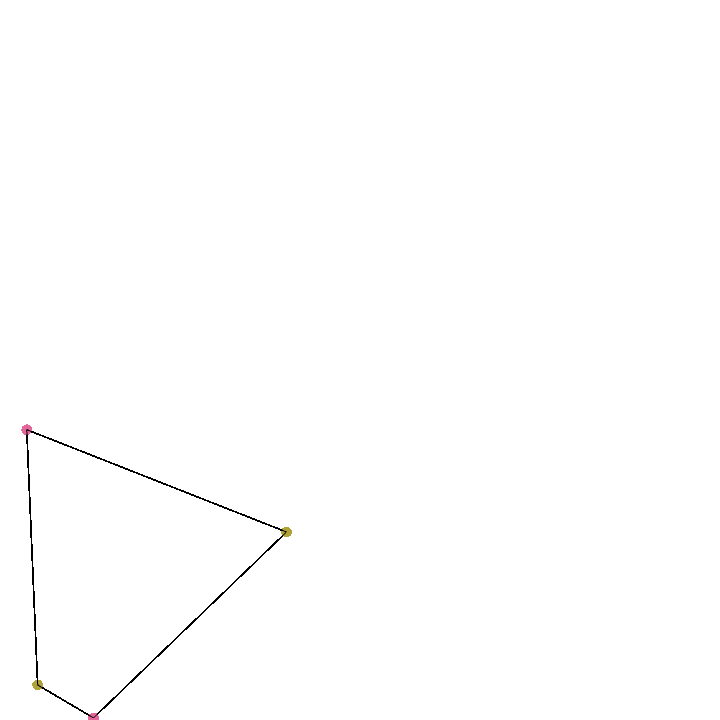
\includegraphics[width=\linewidth]{./images/no-bridge-wt.png}}
            \end{minipage}
            \hspace{\fill}
            \begin{minipage}{0.3\textwidth}
            \colorbox{gray}{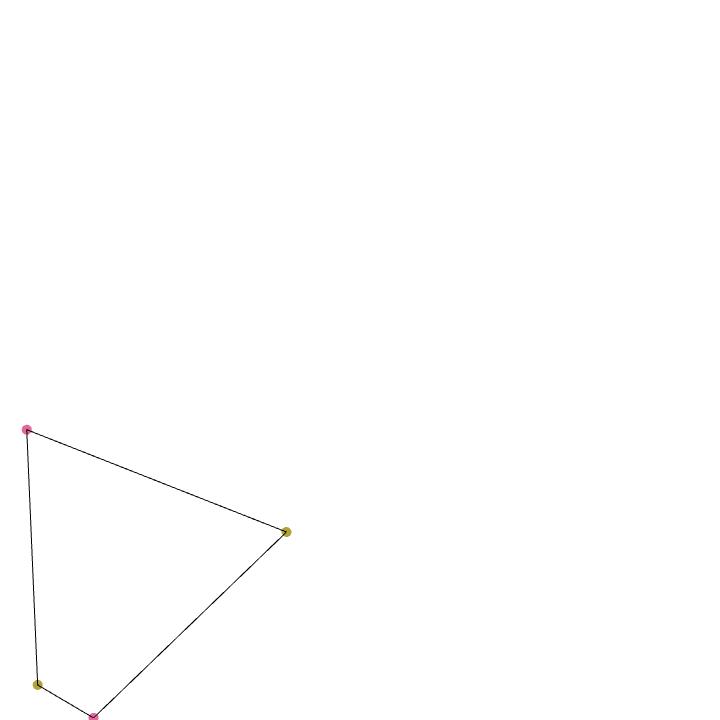
\includegraphics[width=\linewidth]{./images/backbone-wt.png}}
            \end{minipage}
            \hspace{\fill}
            \begin{minipage}{0.3\textwidth}
            \colorbox{gray}{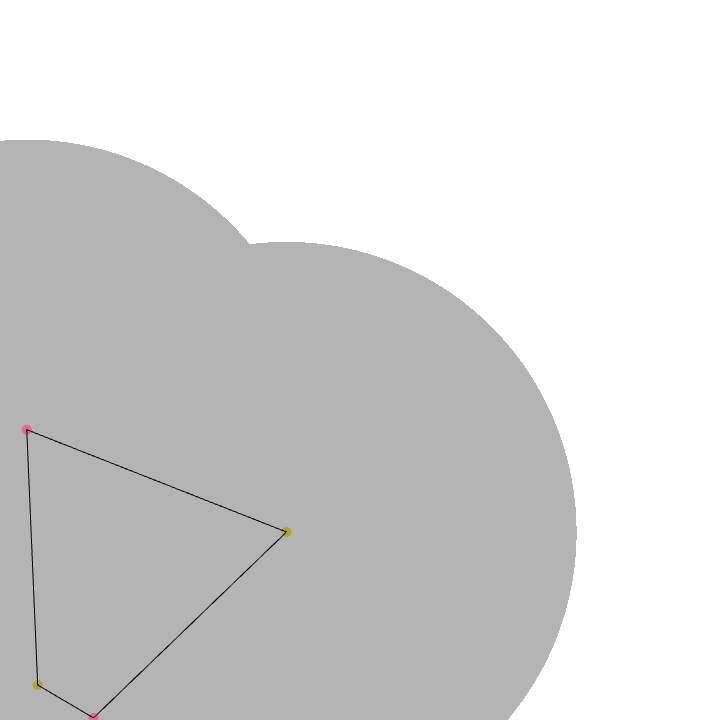
\includegraphics[width=\linewidth]{./images/backbone-coverage-wt.png}}
            \end{minipage}

            \caption{Backbone determination walkthrough for two largest color sets. top left: bipartite subgraph, top center: tails removed, top right: major component, bottom left: bridges and minor blocks removed, bottom center: final backbone, bottom right: coverage area}
            \label{wtbackbone}
        \end{figure}

    \subsection{Verification}

        \subsubsection{Node Placement and Edge Determination}
        The nodes can be verified to be distributed uniformly if the degrees follow a normal distribution. To show that the distribution of degrees for each of the geometries are following a normal distribution, the degree histograms are plotted for each of the benchmarks. The histrograms for Square are given in Figure \ref{squaredeghists}, Disk are given in Figure \ref{diskdeghists}, and Sphere are given in Figure \ref{spheredeghists}. These histograms clearly follow a normal distribution, so the nodes must be placed uniformly.

        \subsubsection{Graph Coloring}
        Smallest-last vertex ordering can be verified by looking at the difference between the degree of nodes in the original graph and when they are deleted in smallest-last vertex ordering. Since smallest-last vertex ordering starts with the original representation of the graph, and repeatedly removed nodes until the graph is empty, it would be expected that the distribution of degrees when deleted diverges from the original distribution of degrees. As can be seen in Figures \ref{squaredegdelhists}, \ref{diskdegdelhists}, and \ref{spheredegdelhists}, this is exactly the case. The original degree of nodes is given in green and the degree when deleted in SLVO is given in blue. The two distributions start out at the same value (on the end of +x, which is the first vertex removed in SLVO). The degree of nodes when deleted then settles onto a lower average than the original degree of nodes because edges are always being removed. Also. the degree of nodes when deleted has a much more consistent upper bound than the original degree of nodes because the node with the fewest number of neighbors is always removed in each step of smallest-last vertex ordering. This will cause the fewest number of nodes to move to the next lowest bucket, so the bulk of the nodes should have a relatively large degree when deleted.
        \par
        Some other interesting features about these graphs are the drops to zero degree when deleted for some nodes in the middle of smallest-last vertex ordering. Whenever this happens, it indicates that the removal of some node caused the creation of a new component. Since the node would have its neighbors moved to the next lowest bucket, they would likely be picked for deletion in the next iteration. This feature shows SLVO removing these minor components before returning to the original graph to continue deletions.
        \par
        It can also be seen where the terminal clique is found on most of the graphs in Figures \ref{squaredegdelhists}, \ref{diskdegdelhists}, and \ref{spheredegdelhists}. Since the terminal clique is the last set of nodes to be deleted, we look to vertex 0. It can be seen most notably in the benchmark for Square 0 in Figures \ref{squaredegdelhists} that there is a peak in the degree when deleted during SLVO and then a gradual tapering down of the degree of the remaining nodes until the degree of the last node is zero and it is removed. This is consistent with the expected behavior of smallest-last vertex ordering, and indicates that the measured values for terminal clique size are correct.
        \par
        The color sets can be verified by looking at the distribution of colors used to color the graph. The number of items in each color should follow a trend where the first colors used have the most members, and the last colors have the fewest items because they are used to accommodate nodes where the earlier colors are all used by a node's neighbors. This trend is shown in Figures \ref{squarecolorhists}, \ref{diskcolorhists}, and \ref{spherecolorshists}.
        \par
        To further verify the accuracy of the smallest-last coloring implementation additional code was used to verify that the coloring result was correct while running benchmarks. All of the nodes in the smallest-last vertex ordering are traversed, and for each node, the edges are visited to see if any adjacent nodes have the same color as the node being checked. If any of these neighbors have the same color, the coloring is not correct and our independent sets cannot be used for backbone determination. All of the benchmarks ran and returned valid colorings.

        \subsubsection{Backbone Determination}
        The runtime for the backbone determination method can be verified by varying the number of nodes and measuring the runtime of the algorithm. By looking at how the runtime grows, we can calculate the trend line that best fits the growth rate. For the first comparison, the number of nodes is varied from 4,000 to 64,000 in steps of 4,000, while holding the desired average degree constant at 16. As we can see in Figure \ref{runtime}, the growth rates of the runtime of backbone determination follow a linear trend for each of the topologies. The trend line functions are given on the graph.
        \par
        For the second metric, the number of nodes is held constant at 32,000 and the desired average degree is varied from 2 to 32 in steps of 2. The graph is given in Figure \ref{runtime}. It can be seen that the runtimes for this test follow a linear trend for each of the topologies.
        \par
        To further verify the integrity of the generated backbones, the final backbones for each topology are given in Figures \ref{squaresa}, \ref{squaresb}, \ref{disks}, and \ref{spheres}. Information on the colors used, order, size, domination, and number of faces are given in \ref{tab3}. It can be seen that there are no nodes with only one neighbor, and each block of nodes has multiple connections to the rest of the backbone. This verifies that if one node were to fail there would still be a path connecting all remaining nodes.
        \par
        All of the backbones are examples of Gabriel Graphs. Given some edge between two nodes A and B, A and B are Gabriel neighbors if there are no other nodes within a circle that has a diameter of edge AB. If the entire graph is comprised of Gabriel neighbors, then the graph is a Gabriel Graph \cite{rggpartition}. Since the maximum connection radius of a node is predetermined, and all nodes within that connection radius to a certain node are connected to that node, all edges in the graph must represent Grabriel neighbors. Because the bipartite subgraphs are created by pairing two independent color sets, and because a single color set cannot have any connections to itself, if two color sets are paired it is guaranteed that a circle drawn circumscribing those nodes will not include any other nodes in that region becuase that extra node would have to share a connection edge with both of the nodes on the diameter of the circle which would make the coloring invalid. Since the colorings have been verified to be correct, these bipartite subgraphs must be Gabriel graphs and therefore must be planar.

\section{Results Summary}
This report details all of the algorithms used, and their Python implementations for generating, coloring, and determining a backbone of a wireless sensor network modeled by a random geometric graph. The simulation is implemented in linear time which makes it easily scalable to different parameters, including the order of the graph and the desired number of neighbors for each sensor. Additionally, the implementation is easy to extend to different topologies by subclassing the Topology or Sphere classes and overriding the method for generating nodes (generateNodes) and calculating the radius for the desired number of neighbors (\_getRadiusForAverageDegree).
\par
The linear runtime of the simulation is shown in the runtime graphs in Figure \ref{runtime}. All of the algorithms together run in linear ($O(n)$) time. The two-dimensional topologies have a smaller constant multiplier on the linear runtime than the three-dimensional topology because of the added spatial dimension of the sphere. Additionally, the cell method for determining graph edges is more efficient in 2D space because the cells extend to be rectangular prisms in 3D space. This means nodes are tested as possible neighbors that appear on opposite ends of the graph. Regardless, the simulation is highly-scalable and produces high-coverage, fault-tolerant backbones.

\newpage

\begin{thebibliography}{13}
    \bibitem{rggpartition}
    Chen, Zizhen; Matula, David, Bipartite Grid Partitioning of a Random Geometric Graph, 2017

    \bibitem{slv}
    Matula, David; Beck, Leland, Smallest-Last Ordering and Clustering and Graph Coloring Algorithms, 1983

    \bibitem{ian}
    Johnson, Ian, Linear-Time Computation of High-Converage Backbones for Wireless Sensor Networks, https://github.com/ianjjohnson/SensorNetwork/blob/master/Report/Report.pdf, 2016

    \bibitem{processing}
    Fry, Ben; Reas Casey, Processing, https://processing.org, 2018 v3.3.7

    \bibitem{matplotlib}
    The Matplotlib Development, matplotlib, https://matplotlib.org, 2018

    \bibitem{spherepoints}
    Weisstein, Eric W., Wolfram MathWorld Sphere Point Picking, http://mathworld.wolfram.com/SpherePointPicking.html

    \bibitem{spherecap}
    Weisstein, Eric W., Wolfram MathWorld Spherical Cap, http://mathworld.wolfram.com/SphericalCap.html

    \bibitem{euler}
    Weisstein, Eric W., Wolfram MathWorld Polyhedral Formula, http://mathworld.wolfram.com/PolyhedralFormula.html

    \bibitem{bridges}
    Kogler, Jakob, Finding bridges in a graph in $O(N + M)$, https://e-maxx-eng.appspot.com/graph/bridge-searching.html, 2018

    \bibitem{listsort}
    Peters, Tim, Timsort, http://svn.python.org/projects/python/trunk/Objects/listsort.txt

    \bibitem{dictresize}
    Rees, Gareth, Python's underlying hash data structure for dictionaries, https://stackoverflow.com/questions/4279358/pythons-underlying-hash-data-structure-for-dictionaries, 2010

    \bibitem{tupletiming}
    Thomas, Alec, Why is tuple faster than list?, https://stackoverflow.com/questions/3340539/why-is-tuple-faster-than-list, 2010

    \bibitem{fortiming}
    Kruse, Lars, Python Speed, Performance Tips, https://wiki.python.org/moin/PythonSpeed/PerformanceTips, 2016

\end{thebibliography}

\newpage

\section{Appendix A - Figures}

\begin{figure}[h]
    \begin{minipage}{0.48\textwidth}
    \colorbox{gray}{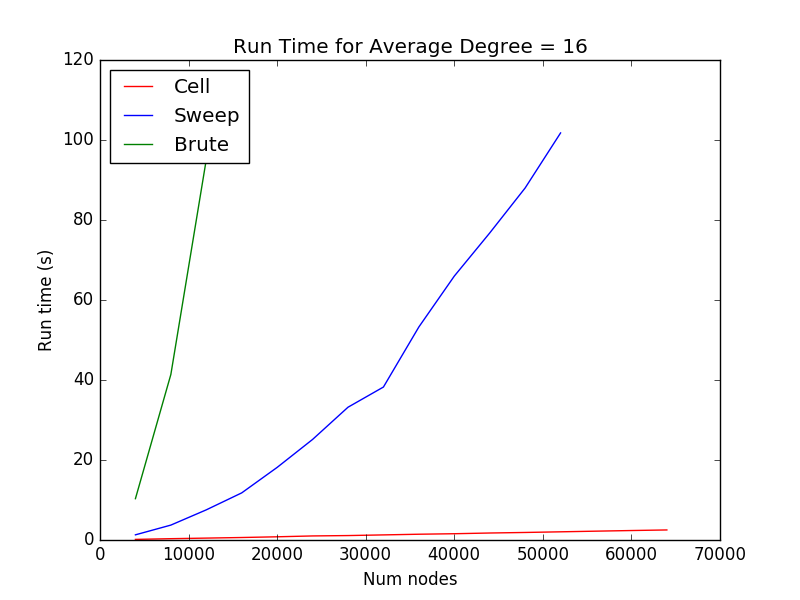
\includegraphics[width=\linewidth]{./graphs/run_time_avg_deg_16.png}}
    \end{minipage}
    \hspace{\fill}
    \begin{minipage}{0.48\textwidth}
    \colorbox{gray}{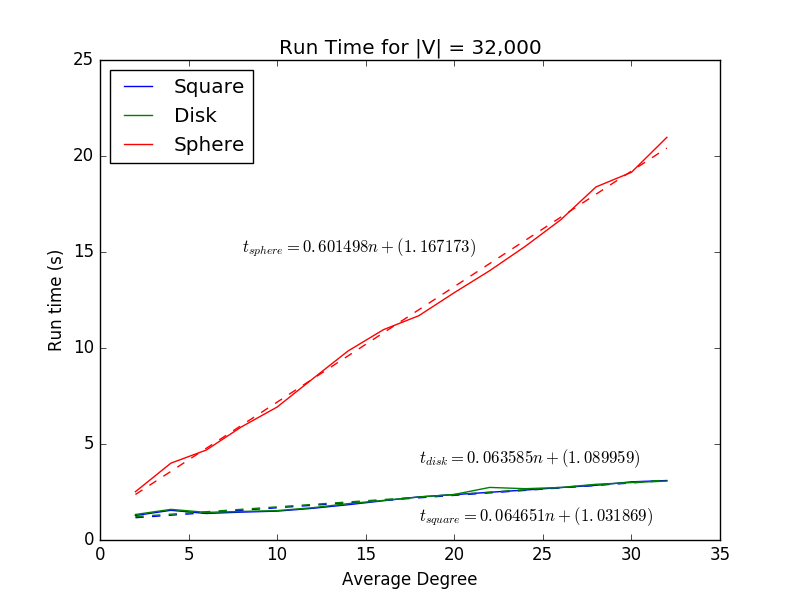
\includegraphics[width=\linewidth]{./graphs/run_time_var_avg_deg.png}}
    \end{minipage}

    \caption{Runtime for backbone determination. left: constant average degree of 16, right: variable average degree}
    \label{runtime}
\end{figure}

\begin{figure}
    \begin{minipage}{0.3\textwidth}
    \colorbox{gray}{\includegraphics[width=\linewidth]{./graphs/hist_deg_square_0.png}}
    \end{minipage}
    \hspace{\fill}
    \begin{minipage}{0.3\textwidth}
    \colorbox{gray}{\includegraphics[width=\linewidth]{./graphs/hist_deg_square_1.png}}
    \end{minipage}
    \hspace{\fill}
    \begin{minipage}{0.3\textwidth}
    \colorbox{gray}{\includegraphics[width=\linewidth]{./graphs/hist_deg_square_2.png}}
    \end{minipage}
    \vskip 0.1in
    \begin{minipage}{0.3\textwidth}
    \colorbox{gray}{\includegraphics[width=\linewidth]{./graphs/hist_deg_square_3.png}}
    \end{minipage}
    \hspace{\fill}
    \begin{minipage}{0.3\textwidth}
    \colorbox{gray}{\includegraphics[width=\linewidth]{./graphs/hist_deg_square_4.png}}
    \end{minipage}
    \hspace{\fill}
    \begin{minipage}{0.3\textwidth}
    \colorbox{gray}{\includegraphics[width=\linewidth]{./graphs/hist_deg_square_5.png}}
    \end{minipage}
    \vskip 0.1in
    \begin{minipage}{0.3\textwidth}
    \colorbox{gray}{\includegraphics[width=\linewidth]{./graphs/hist_deg_square_6.png}}
    \end{minipage}
    \hspace{\fill}

    \caption{Square benchmarks distribution of degree graphs}
    \label{squaredeghists}
\end{figure}

\begin{figure}
    \begin{minipage}{0.45\textwidth}
    \colorbox{gray}{\includegraphics[width=\linewidth]{./graphs/hist_deg_disk_0.png}}
    \end{minipage}
    \hspace{\fill}
    \begin{minipage}{0.45\textwidth}
    \colorbox{gray}{\includegraphics[width=\linewidth]{./graphs/hist_deg_disk_1.png}}
    \end{minipage}
    \vskip 0.25in
    \begin{minipage}{0.45\textwidth}
    \colorbox{gray}{\includegraphics[width=\linewidth]{./graphs/hist_deg_disk_2.png}}
    \end{minipage}

    \caption{Disk benchmarks distribution of degree graphs}
    \label{diskdeghists}
\end{figure}

\begin{figure}
    \begin{minipage}{0.45\textwidth}
    \colorbox{gray}{\includegraphics[width=\linewidth]{./graphs/hist_deg_sphere_0.png}}
    \end{minipage}
    \hspace{\fill}
    \begin{minipage}{0.45\textwidth}
    \colorbox{gray}{\includegraphics[width=\linewidth]{./graphs/hist_deg_sphere_1.png}}
    \end{minipage}
    \vskip 0.25in
    \begin{minipage}{0.45\textwidth}
    \colorbox{gray}{\includegraphics[width=\linewidth]{./graphs/hist_deg_sphere_2.png}}
    \end{minipage}

    \caption{Sphere benchmarks distribution of degree graphs}
    \label{spheredeghists}
\end{figure}

\begin{figure}
    \begin{minipage}{0.3\textwidth}
    \colorbox{gray}{\includegraphics[width=\linewidth]{./graphs/hist_deg_del_square_0.png}}
    \end{minipage}
    \hspace{\fill}
    \begin{minipage}{0.3\textwidth}
    \colorbox{gray}{\includegraphics[width=\linewidth]{./graphs/hist_deg_del_square_1.png}}
    \end{minipage}
    \hspace{\fill}
    \begin{minipage}{0.3\textwidth}
    \colorbox{gray}{\includegraphics[width=\linewidth]{./graphs/hist_deg_del_square_2.png}}
    \end{minipage}
    \vskip 0.1in
    \begin{minipage}{0.3\textwidth}
    \colorbox{gray}{\includegraphics[width=\linewidth]{./graphs/hist_deg_del_square_3.png}}
    \end{minipage}
    \hspace{\fill}
    \begin{minipage}{0.3\textwidth}
    \colorbox{gray}{\includegraphics[width=\linewidth]{./graphs/hist_deg_del_square_4.png}}
    \end{minipage}
    \hspace{\fill}
    \begin{minipage}{0.3\textwidth}
    \colorbox{gray}{\includegraphics[width=\linewidth]{./graphs/hist_deg_del_square_5.png}}
    \end{minipage}
    \vskip 0.1in
    \begin{minipage}{0.3\textwidth}
    \colorbox{gray}{\includegraphics[width=\linewidth]{./graphs/hist_deg_del_square_6.png}}
    \end{minipage}
    \hspace{\fill}

    \caption{Square benchmarks distribution of degree when deleted graphs}
    \label{squaredegdelhists}
\end{figure}

\begin{figure}
    \begin{minipage}{0.45\textwidth}
    \colorbox{gray}{\includegraphics[width=\linewidth]{./graphs/hist_deg_del_disk_0.png}}
    \end{minipage}
    \hspace{\fill}
    \begin{minipage}{0.45\textwidth}
    \colorbox{gray}{\includegraphics[width=\linewidth]{./graphs/hist_deg_del_disk_1.png}}
    \end{minipage}
    \vskip 0.25in
    \begin{minipage}{0.45\textwidth}
    \colorbox{gray}{\includegraphics[width=\linewidth]{./graphs/hist_deg_del_disk_2.png}}
    \end{minipage}

    \caption{Disk benchmarks distribution of degree when deleted graphs}
    \label{diskdegdelhists}
\end{figure}

\begin{figure}
    \begin{minipage}{0.45\textwidth}
    \colorbox{gray}{\includegraphics[width=\linewidth]{./graphs/hist_deg_del_sphere_0.png}}
    \end{minipage}
    \hspace{\fill}
    \begin{minipage}{0.45\textwidth}
    \colorbox{gray}{\includegraphics[width=\linewidth]{./graphs/hist_deg_del_sphere_1.png}}
    \end{minipage}
    \vskip 0.25in
    \begin{minipage}{0.45\textwidth}
    \colorbox{gray}{\includegraphics[width=\linewidth]{./graphs/hist_deg_del_sphere_2.png}}
    \end{minipage}

    \caption{Sphere benchmarks distribution of degree when deleted graphs}
    \label{spheredegdelhists}
\end{figure}

\begin{figure}
    \begin{minipage}{0.3\textwidth}
    \colorbox{gray}{\includegraphics[width=\linewidth]{./graphs/hist_colors_square_0.png}}
    \end{minipage}
    \hspace{\fill}
    \begin{minipage}{0.3\textwidth}
    \colorbox{gray}{\includegraphics[width=\linewidth]{./graphs/hist_colors_square_1.png}}
    \end{minipage}
    \hspace{\fill}
    \begin{minipage}{0.3\textwidth}
    \colorbox{gray}{\includegraphics[width=\linewidth]{./graphs/hist_colors_square_2.png}}
    \end{minipage}
    \vskip 0.1in
    \begin{minipage}{0.3\textwidth}
    \colorbox{gray}{\includegraphics[width=\linewidth]{./graphs/hist_colors_square_3.png}}
    \end{minipage}
    \hspace{\fill}
    \begin{minipage}{0.3\textwidth}
    \colorbox{gray}{\includegraphics[width=\linewidth]{./graphs/hist_colors_square_4.png}}
    \end{minipage}
    \hspace{\fill}
    \begin{minipage}{0.3\textwidth}
    \colorbox{gray}{\includegraphics[width=\linewidth]{./graphs/hist_colors_square_5.png}}
    \end{minipage}
    \vskip 0.1in
    \begin{minipage}{0.3\textwidth}
    \colorbox{gray}{\includegraphics[width=\linewidth]{./graphs/hist_colors_square_6.png}}
    \end{minipage}
    \hspace{\fill}

    \caption{Square benchmarks distribution of colors graphs}
    \label{squarecolorhists}
\end{figure}

\begin{figure}
    \begin{minipage}{0.45\textwidth}
    \colorbox{gray}{\includegraphics[width=\linewidth]{./graphs/hist_colors_disk_0.png}}
    \end{minipage}
    \hspace{\fill}
    \begin{minipage}{0.45\textwidth}
    \colorbox{gray}{\includegraphics[width=\linewidth]{./graphs/hist_colors_disk_1.png}}
    \end{minipage}
    \vskip 0.25in
    \begin{minipage}{0.45\textwidth}
    \colorbox{gray}{\includegraphics[width=\linewidth]{./graphs/hist_colors_disk_2.png}}
    \end{minipage}

    \caption{Disk benchmarks distribution of colors graphs}
    \label{diskcolorhists}
\end{figure}

\begin{figure}
    \begin{minipage}{0.45\textwidth}
    \colorbox{gray}{\includegraphics[width=\linewidth]{./graphs/hist_colors_sphere_0.png}}
    \end{minipage}
    \hspace{\fill}
    \begin{minipage}{0.45\textwidth}
    \colorbox{gray}{\includegraphics[width=\linewidth]{./graphs/hist_colors_sphere_1.png}}
    \end{minipage}
    \vskip 0.25in
    \begin{minipage}{0.45\textwidth}
    \colorbox{gray}{\includegraphics[width=\linewidth]{./graphs/hist_colors_sphere_2.png}}
    \end{minipage}

    \caption{Sphere benchmarks distribution of colors graphs}
    \label{spherecolorshists}
\end{figure}

% square images

\begin{figure}
    \begin{minipage}{0.3\textwidth}
    \colorbox{gray}{\includegraphics[width=\linewidth]{./images/square_0.png}}
    \end{minipage}
    \hspace{\fill}
    \begin{minipage}{0.3\textwidth}
    \colorbox{gray}{\includegraphics[width=\linewidth]{./images/square_0_bb_0.png}}
    \end{minipage}
    \hspace{\fill}
    \begin{minipage}{0.3\textwidth}
    \colorbox{gray}{\includegraphics[width=\linewidth]{./images/square_0_bb_1.png}}
    \end{minipage}
    \vskip 0.1in
    \begin{minipage}{0.3\textwidth}
    \colorbox{gray}{\includegraphics[width=\linewidth]{./images/square_1.png}}
    \end{minipage}
    \hspace{\fill}
    \begin{minipage}{0.3\textwidth}
    \colorbox{gray}{\includegraphics[width=\linewidth]{./images/square_1_bb_0.png}}
    \end{minipage}
    \hspace{\fill}
    \begin{minipage}{0.3\textwidth}
    \colorbox{gray}{\includegraphics[width=\linewidth]{./images/square_1_bb_1.png}}
    \end{minipage}
    \vskip 0.1in
    \begin{minipage}{0.3\textwidth}
    \colorbox{gray}{\includegraphics[width=\linewidth]{./images/square_2.png}}
    \end{minipage}
    \hspace{\fill}
    \begin{minipage}{0.3\textwidth}
    \colorbox{gray}{\includegraphics[width=\linewidth]{./images/square_2_bb_0.png}}
    \end{minipage}
    \hspace{\fill}
    \begin{minipage}{0.3\textwidth}
    \colorbox{gray}{\includegraphics[width=\linewidth]{./images/square_2_bb_1.png}}
    \end{minipage}
    \vskip 0.1in
    \begin{minipage}{0.3\textwidth}
    \colorbox{gray}{\includegraphics[width=\linewidth]{./images/square_3.png}}
    \end{minipage}
    \hspace{\fill}
    \begin{minipage}{0.3\textwidth}
    \colorbox{gray}{\includegraphics[width=\linewidth]{./images/square_3_bb_0.png}}
    \end{minipage}
    \hspace{\fill}
    \begin{minipage}{0.3\textwidth}
    \colorbox{gray}{\includegraphics[width=\linewidth]{./images/square_3_bb_1.png}}
    \end{minipage}

    \caption{Square benchmark graphs and backbones}
    \label{squaresa}
\end{figure}

\begin{figure}
    \begin{minipage}{0.3\textwidth}
    \colorbox{gray}{\includegraphics[width=\linewidth]{./images/square_4.png}}
    \end{minipage}
    \hspace{\fill}
    \begin{minipage}{0.3\textwidth}
    \colorbox{gray}{\includegraphics[width=\linewidth]{./images/square_4_bb_0.png}}
    \end{minipage}
    \hspace{\fill}
    \begin{minipage}{0.3\textwidth}
    \colorbox{gray}{\includegraphics[width=\linewidth]{./images/square_4_bb_1.png}}
    \end{minipage}
    \vskip 0.1in
    \begin{minipage}{0.3\textwidth}
    \colorbox{gray}{\includegraphics[width=\linewidth]{./images/square_5.png}}
    \end{minipage}
    \hspace{\fill}
    \begin{minipage}{0.3\textwidth}
    \colorbox{gray}{\includegraphics[width=\linewidth]{./images/square_5_bb_0.png}}
    \end{minipage}
    \hspace{\fill}
    \begin{minipage}{0.3\textwidth}
    \colorbox{gray}{\includegraphics[width=\linewidth]{./images/square_5_bb_1.png}}
    \end{minipage}
    \vskip 0.1in
    \begin{minipage}{0.3\textwidth}
    \colorbox{gray}{\includegraphics[width=\linewidth]{./images/square_6.png}}
    \end{minipage}
    \hspace{\fill}
    \begin{minipage}{0.3\textwidth}
    \colorbox{gray}{\includegraphics[width=\linewidth]{./images/square_6_bb_0.png}}
    \end{minipage}
    \hspace{\fill}
    \begin{minipage}{0.3\textwidth}
    \colorbox{gray}{\includegraphics[width=\linewidth]{./images/square_6_bb_1.png}}
    \end{minipage}
    \vskip 0.1in

    \caption{Square benchmark graphs and backbones}
    \label{squaresb}
\end{figure}

% disk images

\begin{figure}
    \begin{minipage}{0.3\textwidth}
    \colorbox{gray}{\includegraphics[width=\linewidth]{./images/disk_0.png}}
    \end{minipage}
    \hspace{\fill}
    \begin{minipage}{0.3\textwidth}
    \colorbox{gray}{\includegraphics[width=\linewidth]{./images/disk_0_bb_0.png}}
    \end{minipage}
    \hspace{\fill}
    \begin{minipage}{0.3\textwidth}
    \colorbox{gray}{\includegraphics[width=\linewidth]{./images/disk_0_bb_1.png}}
    \end{minipage}
    \vskip 0.1in
    \begin{minipage}{0.3\textwidth}
    \colorbox{gray}{\includegraphics[width=\linewidth]{./images/disk_1.png}}
    \end{minipage}
    \hspace{\fill}
    \begin{minipage}{0.3\textwidth}
    \colorbox{gray}{\includegraphics[width=\linewidth]{./images/disk_1_bb_0.png}}
    \end{minipage}
    \hspace{\fill}
    \begin{minipage}{0.3\textwidth}
    \colorbox{gray}{\includegraphics[width=\linewidth]{./images/disk_1_bb_1.png}}
    \end{minipage}
    \vskip 0.1in
    \begin{minipage}{0.3\textwidth}
    \colorbox{gray}{\includegraphics[width=\linewidth]{./images/disk_2.png}}
    \end{minipage}
    \hspace{\fill}
    \begin{minipage}{0.3\textwidth}
    \colorbox{gray}{\includegraphics[width=\linewidth]{./images/disk_2_bb_0.png}}
    \end{minipage}
    \hspace{\fill}
    \begin{minipage}{0.3\textwidth}
    \colorbox{gray}{\includegraphics[width=\linewidth]{./images/disk_2_bb_1.png}}
    \end{minipage}
    \vskip 0.1in

    \caption{Disk benchmark graphs and backbones}
    \label{disks}
\end{figure}

% sphere images

\begin{figure}
    \begin{minipage}{0.3\textwidth}
    \colorbox{gray}{\includegraphics[width=\linewidth]{./images/sphere_0.png}}
    \end{minipage}
    \hspace{\fill}
    \begin{minipage}{0.3\textwidth}
    \colorbox{gray}{\includegraphics[width=\linewidth]{./images/sphere_0_bb_0.png}}
    \end{minipage}
    \hspace{\fill}
    \begin{minipage}{0.3\textwidth}
    \colorbox{gray}{\includegraphics[width=\linewidth]{./images/sphere_0_bb_1.png}}
    \end{minipage}
    \vskip 0.1in
    \begin{minipage}{0.3\textwidth}
    \colorbox{gray}{\includegraphics[width=\linewidth]{./images/sphere_1.png}}
    \end{minipage}
    \hspace{\fill}
    \begin{minipage}{0.3\textwidth}
    \colorbox{gray}{\includegraphics[width=\linewidth]{./images/sphere_1_bb_0.png}}
    \end{minipage}
    \hspace{\fill}
    \begin{minipage}{0.3\textwidth}
    \colorbox{gray}{\includegraphics[width=\linewidth]{./images/sphere_1_bb_1.png}}
    \end{minipage}
    \vskip 0.1in
    \begin{minipage}{0.3\textwidth}
    \colorbox{gray}{\includegraphics[width=\linewidth]{./images/sphere_2.png}}
    \end{minipage}
    \hspace{\fill}
    \begin{minipage}{0.3\textwidth}
    \colorbox{gray}{\includegraphics[width=\linewidth]{./images/sphere_2_bb_0.png}}
    \end{minipage}
    \hspace{\fill}
    \begin{minipage}{0.3\textwidth}
    \colorbox{gray}{\includegraphics[width=\linewidth]{./images/sphere_2_bb_1.png}}
    \end{minipage}
    \vskip 0.1in

    \caption{Sphere benchmark graphs and backbones}
    \label{spheres}
\end{figure}

\newpage

\section{Appendix B - Code Listings}

\lstset{style=codestyle}

\lstinputlisting[language=Python, caption=Processing driver]{../Processing/Processing.pyde}

\lstinputlisting[language=Python, caption=Topology class and subclasses]{../Processing/objects/topology.py}

\end{document}
